\باب{تکمل کے طریقے}
ہم نے دیکھا کہ چیزوں کی ناپ اور روز مرہ زندگی کے اعمال کی نمونہ کشی تکمل کو جنم دیتے ہیں۔ ہم جانتے ہیں کہ الٹ تفرق سے تکمل کو حل کیا جا سکتا ہے۔کسی عمل کی نمونہ کشی میں زیادہ گہرائی تک جانے سے زیادہ پیچیدہ تکمل حاصل ہوتا ہے۔ ہم جاننا چاہتے ہیں کہ اس طرح کے پیچیدہ تکمل کو کس طرح سادہ صورت دی جا سکتی ہے جن کے ساتھ کام کرنا آسان ہو۔ اس باب میں ہم انجانے تکمل سے جانے پہچانے تکمل کا حصول سیکھیں گے جنہیں جدول سے دیکھا جا سکتا ہے یا جس کو کمپیوٹر سے حل کیا جا سکتا ہے۔

\حصہ{تکمل کے بنیادی کلیات}   
ہم نے حصہ \حوالہ{حصہ_تکمل_غیر_قطعی_تکمل} میں دیکھا کہ غیر قطعی تکمل کو حل کرنے کے لئے اس کے الٹ تفرق کے ساتھ مستقل جمع کرنا ہو گا۔ جدول \حوالہ{جدول_طریقے_تکمل_بنیادی_کلیات} میں ان  تکمل کی بنیادی روپ درج کی گئی ہے جنہیں اب تک ہم حل کرتے آ رہے ہیں۔ زیادہ تکملات کا جدول کتاب کی آخر میں پیش کیا گیا ہے جس پر حصہ میں غور کیا جائے گا۔

\begin{table}
\caption{تکمل کے بنیادی کلیات}
\label{جدول_طریقے_تکمل_بنیادی_کلیات}
\renewcommand{\arraystretch}{2}
\centering
\begin{tabular}{L|L}
\toprule
\text{شمار}&\text{کلیہ}\\
\midrule
1&\int \dif u=u+C\\
2&\int k\dif u=ku+C \quad \text{\RL{($k$ عدد ہے)}}\\
3&\int(\dif u+\dif v)=\int \dif u+\int \dif v\\
4&\int u^n\dif u=\frac{u^{n+1}}{n+1}+C\quad (n\ne -1)\\
5&\int\frac{\dif u}{u}=\ln \abs{u}+C\\
6&\int\sin u\dif u=-\cos u+C\\
7&\int\cos u\dif u=\sin u+C\\
8&\int \sec^2u\dif u=\tan u +C\\
9&\int \csc^2u\dif u=-\cot u+C\\
10&\int\sec u\tan u\dif u=\sec u+C\\
11&\int \csc u\cot u\dif u=-\csc u+C\\
12&\int \tan u\dif u=-\ln\abs{\cos u}+C=\ln\abs{\sec u}+C\\
13&\int \cot u\dif u=\ln \abs{\sin u}+C=-\ln\abs{\csc u}+C\\
14&\int e^u\dif u=e^u+C\\
15&\int a^u\dif u=\frac{a^u}{\ln a}+C\quad (a>0,\, a\ne 1)\\
16&\int \frac{\dif u}{\sqrt{a^2-u^2}}=\sin^{-1}(\tfrac{u}{a})+C\\
17&\int \frac{\dif u}{a^2+u^2}=\frac{1}{a}\tan^{-1}(\tfrac{u}{a})+C\\
18&\int\frac{\dif u}{u\sqrt{u^2-a^2}}=\frac{1}{a}\sec^{-1}\abs{\tfrac{u}{a}}+C\\
\bottomrule
\end{tabular}
\end{table}
\جزوحصہء{الجبرائی طریقہ}
ہمیں عموماً تکمل کو جانی پہچانی معیاری روپ میں لکھنا ہو گا۔

\ابتدا{مثال}\ترچھا{سادہ روپ حاصل کرنے کا بدل}\\
تکمل \عددی{\int\tfrac{2x-9}{\sqrt{x^2-9x+1}}\dif x} حل کریں۔

حل:
\begin{align*}
\int\frac{2x-9}{\sqrt{x^2-9x+1}}\dif x&=\int\frac{\dif u}{\sqrt{u}}&&u=x^2-9x+1\\
&=\int u^{-1/2}\dif u\\
&=\frac{u^{(-1/2)+1}}{(-1/2)+1}+C&&\text{\RL{جدول \حوالہ{جدول_طریقے_تکمل_بنیادی_کلیات} کلیہ $4$ میں $n=-1/2$}}\\
&=2u^{1/2}+C\\
&=2\sqrt{x^2-9x+1}+C
\end{align*}
\انتہا{مثال}
%================
\ابتدا{مثال}\ترچھا{تکمیل مربع}\\
تکمل \عددی{\int\tfrac{\dif x}{\sqrt{8x-x^2}}} حل کریں۔

حل:\quad
ہم مربع مکمل کرتے ہوئے زیر جذر کو لکھتے ہیں:
\begin{align*}
8x-x^2&=-(x^2-8x)=-(x^2-8x+16-16)\\
&=-(x^2-8x+16)+16=16-(x-4)^2
\end{align*}
\begin{align*}
\int\frac{\dif x}{\sqrt{8x-x^2}}&=\int\frac{\dif x}{\sqrt{16-(x-4)^2}}\\
&=\int\frac{\dif u}{\sqrt{a^2-u^2}}&&a=4,u=(x-4)\\
&=\sin^{-1}(\tfrac{u}{a})+C&&\text{\RL{جدول \حوالہ{جدول_طریقے_تکمل_بنیادی_کلیات} کلیہ $16$}}\\
&=\sin^{-1}(\tfrac{x-4}{4})+C
\end{align*}
\انتہا{مثال}
%================
\ابتدا{مثال}\ترچھا{طاقت پھیلا کر تماثل کا استعمال}\\
تکمل \عددی{\int(\sec x\tan x)^2\dif x} حل کریں۔

حل:\quad
ہم متکمل کو پھیلاتے ہیں۔
\begin{align*}
(\sec x+\tan x)^2=\sec^2x+2\sec x\tan x+\tan^2x
\end{align*}
بائیں ہاتھ پہلے دو اجزاء کا تکمل ہم جانتے ہیں البتہ \عددی{\tan^2x} کا کچھ کرنا ہو گا۔ ہم درج ذیل تماثل کے ذریعہ اس کو جانی پہچانی روپ میں تبدیل کرتے ہیں۔
\begin{align*}
\tan^2x+1=\sec^2x\quad \implies\quad \tan^2x=\sec^2x-1
\end{align*}
یوں درج ذیل ہو گا۔
\begin{align*}
\int (\sec x+\tan x)^2\dif x&=\int(\sec^2x+2\sec x\tan x+\sec^2x-1)\dif x\\
&=2\int \sec^2\dif x+2\int\sec x\tan x\dif x-\int 1\dif x\\
&=2\tan x+2\sec x-x+C
\end{align*}
\انتہا{مثال}
%=================
\ابتدا{مثال}\ترچھا{جذر سے چھٹکارا}\\
تکمل \عددی{\int_0^{\pi/4}\sqrt{1+\cos 4x}\dif x} حل کریں۔

حل:\quad
ہم تماثل
\begin{align*}
\cos^2\theta=\frac{1+\cos 2\theta}{2}\quad \implies 1+\cos 2\theta=2\cos^2\theta
\end{align*}
میں \عددی{\theta=2x} پر کر کے 
\begin{align*}
1+\cos 4x=2\cos^22x
\end{align*}
لکھتے ہیں۔یوں درج ذیل ہو گا جہاں تیسرے قدم پر وقفہ \عددی{[0,\tfrac{\pi}{4}]} پر \عددی{\cos 2x\ge 0} کی بنا \عددی{\abs{\cos 2x}=\cos 2x} ہو گا۔
\begin{align*}
\int_0^{\pi/4}\sqrt{1+\cos 4x}\dif x&=\int_0^{\pi/4}\sqrt{2}\sqrt{\cos^22x}\dif x\\
&=\sqrt{2}\int_0^{\pi/4}\abs{\cos 2x}\dif x&&\sqrt{u^2}=\abs{u}\\
&=\sqrt{2}\int_0^{\pi/4}\cos 2x\dif x\\
&=\sqrt{2}\left.\frac{\sin 2x}{2}\right\vert_0^{\pi/4}\\
&=\sqrt{2}\big[\frac{1}{2}-0\big]=\frac{\sqrt{2}}{2}
\end{align*}
\انتہا{مثال}
%================
\ابتدا{مثال}\ترچھا{غیر مناسب کسر کی مناسب کسر میں تبدیلی}\\
تکمل \عددی{\int\tfrac{3x^2-7x}{3x+2}\dif x} حل کریں۔

حل:\quad 
متکمل غیر مناسب کسر (نسب نما کی طاقت، شمار کنندہ کی طاقت سے زیادہ یا اس کے برابر ہے)  ہے۔ اس کا تکمل لینے سے پہلے ہم پہلے تقسیم کر کے حاصل تقسیم اور باقی حاصل کرتے ہیں جو مناسب کسر ہو گا:
\begin{align*}
\frac{3x^2-7x}{3x+2}=x-3+\frac{6}{3x+2}
\end{align*}
یوں درج ذیل ہو گا۔
\begin{align*}
\int\frac{3x^2-7x}{3x+2}\dif x=\int\big(x-3+\frac{6}{3x+2}\big)\dif x=\frac{x^2}{2}-3x+2\ln\abs{3x+2}+C
\end{align*}
\انتہا{مثال}
%=================
یہ ضروری نہیں ہے کہ غیر مناسب کسر کو بذریعہ تقسیم مناسب  کسر میں تبدیل کرنے سے  ہمیں ایسا تکمل حاصل ہو جسے ہم سیدھا تکمل کر سکیں۔ ایسی صورت پر حصہ میں غور کیا جائے گا۔

\ابتدا{مثال}\ترچھا{ایک کسر کی علیحدگی}\\
تکمل \عددی{\int\tfrac{3x+2}{\sqrt{1-x^2}}\dif x} حل کریں۔

حل:\quad
ہم متکمل کو دو علیحدہ کسر لکھتے ہیں۔
\begin{align*}
\int\frac{3x+2}{\sqrt{1-x^2}}\dif x=3\int\frac{x\dif x}{\sqrt{1-x^2}}+2\int\frac{\dif x}{\sqrt{1-x^2}}
\end{align*}
بائیں ہاتھ پہلے نئے تکمل میں ہم \عددی{u=1-x^2}، \عددی{\dif u=-2x\dif x} اور \عددی{x\dif x=-\frac{1}{2}\dif u} پر کرتے ہیں۔
\begin{align*}
3\int\frac{x\dif x}{\sqrt{1-x^2}}&=3\int\frac{(-1/2)\dif u}{\sqrt{u}}=-\frac{3}{2}\int u^{-1/2}\dif u\\
&=-\frac{3}{2}\cdot \frac{u^{1/2}}{1/2}+C_1=-3\sqrt{1-x^2}+C_1
\end{align*}
دوسرا نیا تکمل معیاری روپ میں ہے لہٰذا
\begin{align*}
2\int\frac{\dif x}{\sqrt{1-x^2}}=2\sin^{-1}x+C_2
\end{align*} 
ہو گا۔یوں پورا تکمل درج ذیل ہو گا جہاں \عددی{C_1+C_2=C} لکھا گیا ہے۔
\begin{align*}
\int\frac{3x+2}{\sqrt{1-x^2}}\dif x=-3\sqrt{1-x^2}+2\sin^{-1}x+C
\end{align*}

\انتہا{مثال}
%================
\ابتدا{مثال}\شناخت{مثال_طریقے_سیکنٹ_کلیہ_تکمل}\ترچھا{اکائی (\عددی{1}) کی ایک روپ سے ضرب}\\
تکمل \عددی{\int\sec x\dif x} حل کریں۔

حل:
\begin{align*}
\int\sec x\dif x&=\int (\sec x)(1)\dif x\\
&=\int \sec x \cdot \frac{\sec x+\tan x}{\sec x+\tan x}\dif x\\
&=\int \frac{\sec^2x+\sec x\tan x}{\sec x+\tan x}\dif x\\
&=\int\frac{\dif u}{u}&&u=\tan x+\sec x\\
&=\ln \abs{u}+C=\ln\abs{\sec x+\tan x}+C
\end{align*}
\انتہا{مثال}
%===================
\begin{table}
\caption{سیکنٹ اور کوسیکنٹ کے کلیات تکمل}
\label{جدول_طریقے_سیکنٹ_کوسیکنٹ_کلیات}
\centering
\renewcommand{\arraystretch}{2}
\begin{tabular}{L|L}
\toprule
\text{شمار}&\text{کلیہ}\\
\midrule
1&\int \sec u\dif u=\ln \abs{\sec u+\tan u}+C\\
2&\int\csc u\dif u=-\ln\abs{\csc u+\cot u}+C\\
\bottomrule
\end{tabular}
\end{table}

ہم مثال \حوالہ{مثال_طریقے_سیکنٹ_کلیہ_تکمل} کی ترکیب استعمال کرتے ہوئے سیکنٹ اور ٹینجنٹ کی جگہ کوسیکنٹ اور کوٹینجنٹ لیتے ہوئے   کوسیکنٹ کے تکمل کا کلیہ معلوم کر سکتے ہیں (سوال \حوالہ{سوال_طریقے_کوسیکنٹ_تکمل})۔

\موٹا{تکمل کو بنیادی کلیہ کی روپ میں لکھنے کا طریقے}
\begin{align*}
\text{مثال}&&\text{طریقہ}\\
\hline
\frac{2x-9}{\sqrt{x^2-9x+1}}\dif x&=\frac{\dif u}{u}&&\text{\RL{سادہ روپ بذریعہ بدل}}\\
\sqrt{8x-x^2}\dif x&=\sqrt{16-(x-4)^2}&&\text{\RL{تکمیل مربع}}\\
(\sec x+\tan x)^2&=\sec^2x+2\sec x\tan x+\tan^2x&&\text{\RL{تکونیاتی تماثل}}\\
&=\sec^2x+2\sec x\tan x+(\sec^2x-1)\\
&=2\sec^2x+2\sec x\tan x-1\\
\sqrt{1+\cos 4x}&=\sqrt{2\cos^22x}=\sqrt{2}\abs{\cos 2x}&&\text{\RL{جذر سے چھٹکارا}}\\
\frac{3x^2-7x}{3x+2}&=x-3+\frac{6}{3x+2}&&\text{\RL{غیر مناسب سے مناسب کسر کا حصول}}\\
\frac{3x+2}{\sqrt{1-x^2}}&=\frac{3x}{\sqrt{1-x^2}}+\frac{2}{\sqrt{1-x^2}}&&\text{\RL{کسر کی علیحدگی}}\\
\sec x&=\sec x\cdot \frac{\sec x+\tan x}{\sec x+\tan x}&&\text{\RL{اکائی ($1$) کی ایک روپ سے ضرب}}\\
&=\frac{\sec^2x+\sec x\tan x}{\sec x+\tan x}
\end{align*}


%====================================
\حصہء{سوالات}
\موٹا{بنیادی بدل}\\
سوال \حوالہ{سوال_طریقے_بدل_معیاری_روپ_حصول_الف} تا سوال \حوالہ{سوال_طریقے_بدل_معیاری_روپ_حصول_ب} میں بدل کی استعمال سے معیاری روپ حاصل کر کے تکمل حل کریں۔ 

\ابتدا{سوال}\شناخت{سوال_طریقے_بدل_معیاری_روپ_حصول_الف}
$\int\frac{16x\dif x}{\sqrt{8x^2+1}}$\\
جواب:\quad
$2\sqrt{8x^2+1}+C$
\انتہا{سوال}
%======================
\ابتدا{سوال}
$\int\frac{3\cos x\dif x}{\sqrt{1+3\sin x}}$
\انتہا{سوال}
%======================
\ابتدا{سوال}
$\int3\sqrt{\sin v}\cos v\dif v$\\
جواب:\quad
$2(\sin v)^{3/2}+C$
\انتہا{سوال}
%======================
\ابتدا{سوال}
$\int\cot^3y\csc^2y\dif y$
\انتہا{سوال}
%======================
\ابتدا{سوال}
$\int_0^1\frac{16x\dif x}{8x^2+2}$\\
جواب:\quad
$\ln 5$
\انتہا{سوال}
%======================
\ابتدا{سوال}
$\int_{\pi/4}^{\pi/3}\frac{\sec^2z}{\tan z}\dif z$
\انتہا{سوال}
%======================
\ابتدا{سوال}
$\int\frac{\dif x}{\sqrt{x}(\sqrt{x}+1)}$\\
جواب:\quad
$2\ln(\sqrt{x}+1)+C$
\انتہا{سوال}
%======================
\ابتدا{سوال}
$\int\frac{\dif x}{x-\sqrt{x}}$
\انتہا{سوال}
%======================
\ابتدا{سوال}
$\int\cot(3-7x)\dif x$\\
جواب:\quad
$-\tfrac{1}{7}\ln\abs{\sin(3-7x)}+C$
\انتہا{سوال}
%======================
\ابتدا{سوال}
$\int\csc(\pi x-1)\dif x$
\انتہا{سوال}
%======================
\ابتدا{سوال}
$\int e^{\theta}\csc(e^{\theta}+1)\dif \theta$\\
جواب:\quad
$-\ln\abs{\csc(e^{\theta}+1)+\cot(e^{\theta}+1)}+C$
\انتہا{سوال}
%======================
\ابتدا{سوال}
$\int\frac{\cot(3+\ln x)}{x}\dif x$
\انتہا{سوال}
%======================
\ابتدا{سوال}
$\int \sec\frac{t}{3}\dif t$\\
جواب:\quad
$3\ln\abs{\sec\tfrac{t}{3}+\tan\tfrac{t}{3}}+C$
\انتہا{سوال}
%======================
\ابتدا{سوال}
$\int x\sec(x^2-5)\dif x$
\انتہا{سوال}
%======================
\ابتدا{سوال}
$\int\csc(s-\pi)\dif s$\\
جواب:\quad
$-\ln\abs{\csc(s-\pi)+\cot(s-\pi)}+C$
\انتہا{سوال}
%======================
\ابتدا{سوال}
$\int \frac{1}{\theta^2}\csc\frac{1}{\theta}\dif \theta$
\انتہا{سوال}
%======================
\ابتدا{سوال}
$\int_0^{\sqrt{\ln 2}}2xe^{x^2}\dif x$\\
جواب:\quad
$1$
\انتہا{سوال}
%======================
\ابتدا{سوال}
$\int_{\pi/2}^{\pi}\sin(y)e^{\cos y}\dif y$
\انتہا{سوال}
%======================
\ابتدا{سوال}
$\int e^{\tan v}\sec^2v\dif v$\\
جواب:\quad
$e^{\tan v}+C$
\انتہا{سوال}
%======================
\ابتدا{سوال}
$\int\frac{e^{\sqrt{t}}}{\sqrt{t}}\dif t$
\انتہا{سوال}
%======================
\ابتدا{سوال}
$\int 3^{x+1}\dif x$\\
جواب:\quad
$\tfrac{e^{x+1}}{\ln 3}+C$
\انتہا{سوال}
%======================
\ابتدا{سوال}
$\int\frac{2^{\ln x}}{x}\dif x$
\انتہا{سوال}
%======================
\ابتدا{سوال}
$\int\frac{2^{\sqrt{w}}}{2\sqrt{w}}\dif w$\\
جواب:\quad
$\tfrac{2^{\sqrt{w}}}{\ln 2}+C$
\انتہا{سوال}
%======================
\ابتدا{سوال}
$\int 10^{2\theta}\dif \theta$
\انتہا{سوال}
%======================
\ابتدا{سوال}
$\int\frac{9\dif u}{1+9u^2}$\\
جواب:\quad
$3\tan^{-1}3u+C$
\انتہا{سوال}
%======================
\ابتدا{سوال}
$\int\frac{4\dif x}{1+(2x+1)^2}$
\انتہا{سوال}
%======================
\ابتدا{سوال}
$\int_0^{1/6}\frac{\dif x}{\sqrt{1-9x^2}}$\\
جواب:\quad
$\tfrac{\pi}{18}$
\انتہا{سوال}
%======================
\ابتدا{سوال}
$\int_0^1\frac{\dif t}{\sqrt{4-t^2}}$
\انتہا{سوال}
%======================
\ابتدا{سوال}
$\int\frac{2s\dif s}{\sqrt{1-s^4}}$\\
جواب:\quad
$\sin^{-1}s^2+C$
\انتہا{سوال}
%======================
\ابتدا{سوال}
$\int\frac{2\dif x}{x\sqrt{1-4\ln^2 x}}$
\انتہا{سوال}
%======================
\ابتدا{سوال}
$\int\frac{6\dif x}{x\sqrt{25x^2-1}}$\\
جواب:\quad
$6\sec^{-1}\abs{5x}+C$
\انتہا{سوال}
%======================
\ابتدا{سوال}
$\int\frac{\dif r}{r\sqrt{r^2-9}}$
\انتہا{سوال}
%======================
\ابتدا{سوال}
$\int\frac{\dif x}{e^x+e^{-x}}$\\
جواب:\quad
$\tan^{-1}e^x+C$
\انتہا{سوال}
%======================
\ابتدا{سوال}
$\int\frac{\dif y}{\sqrt{e^{2y}-1}}$
\انتہا{سوال}
%======================
\ابتدا{سوال}
$\int_{1}^{e^{\pi/3}}\frac{\dif x}{x\cos(\ln x)}$\\
جواب:\quad
$\ln(2+\sqrt{3})$
\انتہا{سوال}
%======================
\ابتدا{سوال}\شناخت{سوال_طریقے_بدل_معیاری_روپ_حصول_ب}
$\int\frac{\ln x\dif x}{x+4x\ln^2x}$
\انتہا{سوال}
%======================
\موٹا{تکمیل مربع}\\
سوال \حوالہ{سوال_طریقے_تکمیل_مربع_بدل_الف} تا سوال \حوالہ{سوال_طریقے_تکمیل_مربع_بدل_ب} میں مربع مکمل کر کے اور بدل استعمال کرتے ہوئے  معیاری روپ حاصل کر کے تکمل حل کریں۔

\ابتدا{سوال}\شناخت{سوال_طریقے_تکمیل_مربع_بدل_الف}
$\int_1^2\frac{8\dif x}{x^2-2x+2}$\\
جواب:\quad
$2\pi$
\انتہا{سوال}
%=========================
\ابتدا{سوال}
$\int_2^4\frac{2\dif x}{x^2-6x+10}$
\انتہا{سوال}
%=========================
\ابتدا{سوال}
$\int\frac{\dif t}{\sqrt{-t^2+4t-3}}$\\
جواب:\quad
$\sin^{-1}(t-2)+C$
\انتہا{سوال}
%=========================
\ابتدا{سوال}
$\int\frac{\dif\theta}{\sqrt{2\theta-\theta^2}}$
\انتہا{سوال}
%=========================
\ابتدا{سوال}
$\int\frac{\dif x}{(x+1)\sqrt{x^2+2x}}$\\
جواب:\quad
$\sec^{-1}\abs{x+1}+C\,\text{تب}\, \abs{x+1}>1\, \text{جب}$
\انتہا{سوال}
%=========================
\ابتدا{سوال}\شناخت{سوال_طریقے_تکمیل_مربع_بدل_ب}
$\int\frac{\dif x}{(x-2)\sqrt{x^2-4x+3}}$
\انتہا{سوال}
%=========================
\موٹا{تکونیاتی تماثل}\\
سوال \حوالہ{سوال_طریقے_تماثل_بدل_الف} تا سوال \حوالہ{سوال_طریقے_تماثل_بدل_ب} میں تکونیاتی تماثل اور بدل استعمال کرتے ہوئے معیاری روپ حاصل کر کے تکمل حل کریں۔

\ابتدا{سوال}\شناخت{سوال_طریقے_تماثل_بدل_الف}
$\int(\sec x+\cot x)^2\dif x$\\
جواب:\quad
$\tan x-2\ln \abs{\csc x+\cot x}-\cot x-x+C$
\انتہا{سوال}
%==========================
\ابتدا{سوال}
$\int(\csc x-\tan x)^2\dif x$
\انتہا{سوال}
%==========================
\ابتدا{سوال}
$\int \csc x\sin 3x\dif x$\\
جواب:\quad
$x+\sin 2x+C$
\انتہا{سوال}
%==========================
\ابتدا{سوال}\شناخت{سوال_طریقے_تماثل_بدل_ب}
$\int(\sin 3x\cos 2x-\cos 3x\sin 2x)\dif x$
\انتہا{سوال}
%==========================
\موٹا{غیر مناسب کسر}\\
سوال \حوالہ{سوال_طریقے_غیر_مناسب_بدل_الف} تا سوال \حوالہ{سوال_طریقے_غیر_مناسب_بدل_ب} میں غیر مناسب کسر سے مناسب کسر کے حصول اور بدل کے ذریعہ معیاری روپ حاصل کر کے تکمل حل کریں۔

\ابتدا{سوال}\شناخت{سوال_طریقے_غیر_مناسب_بدل_الف}
$\int\frac{x}{x+1}\dif x$\\
جواب:\quad
$x-\ln\abs{x+1}+C$
\انتہا{سوال}
%=======================
\ابتدا{سوال}
$\int\frac{x^2}{x^2+1}\dif x$
\انتہا{سوال}
%=======================
\ابتدا{سوال}
$\int_{\sqrt{2}}^{3}\frac{2x^3}{x^2-1}\dif x$\\
جواب:\quad
$7+\ln 8$
\انتہا{سوال}
%=======================
\ابتدا{سوال}
$\int_{-1}^{3}\frac{4x^2-7}{2x+3}\dif x$
\انتہا{سوال}
%=======================
\ابتدا{سوال}
$\int\frac{4t^3-t^2+16t}{t^2+4}\dif t$\\
جواب:\quad
$2t^2-t+2\tan^{-1}(\tfrac{t}{2})+C$
\انتہا{سوال}
%=======================
\ابتدا{سوال}\شناخت{سوال_طریقے_غیر_مناسب_بدل_ب}
$\int\frac{2\theta^3-7\theta^2+7\theta}{2\theta-5}\dif \theta$
\انتہا{سوال}
%=======================
\موٹا{کسر کی علیحدگی}\\
سوال \حوالہ{سوال_طریقے_کسر_علیحدہ_بدل_الف} تا سوال \حوالہ{سوال_طریقے_کسر_علیحدہ_بدل_ب} میں کسر علیحدہ کر کے بدل کے ذریعہ معیاری روپ حاصل کر کے تکمل حل کریں۔

\ابتدا{سوال}\شناخت{سوال_طریقے_کسر_علیحدہ_بدل_الف}
$\int\frac{1-x}{\sqrt{1-x^2}}\dif x$\\
جواب:\quad
$\sin^{-1}x+\sqrt{1-x^2}+C$
\انتہا{سوال}
%=====================
\ابتدا{سوال}
$\int\frac{x+2\sqrt{x-1}}{2x\sqrt{x-1}}\dif x$
\انتہا{سوال}
%=====================
\ابتدا{سوال}
$\int_0^{\pi/4}\frac{1+\sin x}{\cos^2x}\dif x$\\
جواب:\quad
$\sqrt{2}$
\انتہا{سوال}
%=====================
\ابتدا{سوال}\شناخت{سوال_طریقے_کسر_علیحدہ_بدل_ب}
$\int_0^{1/2}\frac{2-8x}{1+4x^2}\dif x$
\انتہا{سوال}
%=====================
\موٹا{اکائی \عددی{(1)} کی ایک روپ سے ضرب}\\
سوال \حوالہ{سوال_طریقے_اکائی_بدل_الف} تا سوال \حوالہ{سوال_طریقے_اکائی_بدل_ب} میں اکائی کی ایک روپ سے ضرب اور بدل کے ذریعہ معیاری روپ حاصل کر کے تکمل حل کریں۔

\ابتدا{سوال}\شناخت{سوال_طریقے_اکائی_بدل_الف}
$\int\frac{1}{1+\sin x}\dif x$\\
جواب:\quad
$\tan x-\sec x+C$
\انتہا{سوال}
%===================
\ابتدا{سوال}
$\int\frac{1}{1+\cos x}\dif x$
\انتہا{سوال}
%===================
\ابتدا{سوال}
$\int\frac{1}{\sec\theta+\tan\theta}\dif \theta$\\
جواب:\quad
$\ln\abs{1+\sin\theta}+C$
\انتہا{سوال}
%===================
\ابتدا{سوال}
$\int\frac{1}{\csc\theta+\cot\theta}\dif \theta$
\انتہا{سوال}
%===================
\ابتدا{سوال}
$\int\frac{1}{1-\sec x}\dif x$\\
جواب:\quad
$\cot x+x+\csc x+C$
\انتہا{سوال}
%===================
\ابتدا{سوال}\شناخت{سوال_طریقے_اکائی_بدل_ب}
$\int\frac{1}{1-\csc x}\dif x$
\انتہا{سوال}
%===================
\موٹا{جذر سے چھٹکارا}\\
سوال \حوالہ{سوال_طریقے_جذر_چھٹکارا_الف} تا سوال \حوالہ{سوال_طریقے_جذر_چھٹکارا_ب} میں جذر سے چھٹکارے کے بعد تکمل حل کریں۔

\ابتدا{سوال}\شناخت{سوال_طریقے_جذر_چھٹکارا_الف}
$\int_{0}^{2\pi}\sqrt{\frac{1-\cos x}{2}}\dif x$\\
جواب:\quad
$4$
\انتہا{سوال}
%=======================
\ابتدا{سوال}
$\int_0^{\pi}\sqrt{1-\cos 2x}\dif x$
\انتہا{سوال}
%=======================
\ابتدا{سوال}
$\int_{\pi/2}^{\pi}\sqrt{1+\cos 2t}\dif t$\\
جواب:\quad
$\sqrt{2}$
\انتہا{سوال}
%=======================
\ابتدا{سوال}
$\int_{-\pi}^0\sqrt{1+\cos t}\dif t$
\انتہا{سوال}
%=======================
\ابتدا{سوال}
$\int_{-\pi}^0\sqrt{1-\cos^2\theta}\dif \theta$\\
جواب:\quad
$2$
\انتہا{سوال}
%=======================
\ابتدا{سوال}
$\int_{\pi/2}^{\pi}\sqrt{1-\sin^2\theta}\dif\theta$
\انتہا{سوال}
%=======================
\ابتدا{سوال}
$\int_{-\pi/4}^{\pi/4}\sqrt{1+\tan^2y}\dif y$\\
جواب:\quad
$\ln\abs{\sqrt{2}+1}-\ln\abs{\sqrt{2}-1}$
\انتہا{سوال}
%=======================
\ابتدا{سوال}\شناخت{سوال_طریقے_جذر_چھٹکارا_ب}
$\int_{-\pi/4}^{0}\sqrt{\sec^2y-1}\dif y$
\انتہا{سوال}
%=======================
\موٹا{مختلف قسم کے تکمل}\\
سوال \حوالہ{سوال_طریقے_موزوں_طریقہ_الف} تا سوال \حوالہ{سوال_طریقے_موزوں_طریقہ_ب} میں کوئی بھی موزوں طریقہ استعمال کرتے ہوئے تکمل حل کریں۔

\ابتدا{سوال}\شناخت{سوال_طریقے_موزوں_طریقہ_الف}
$\int_{\pi/4}^{3\pi/4}(\csc x-\cot x)^2\dif x$\\
جواب:\quad
$4-\tfrac{\pi}{2}$
\انتہا{سوال}
%=====================
\ابتدا{سوال}
$\int_0^{\pi/4}(\sec x+4\cos x)^2\dif x$
\انتہا{سوال}
%=====================
\ابتدا{سوال}
$\int\cos\theta\csc(\sin\theta)\dif\theta$\\
جواب:\quad
$-\ln\abs{\csc(\sin\theta)+\cot(\sin\theta)}+C$
\انتہا{سوال}
%=====================
\ابتدا{سوال}
$\int(1+\tfrac{1}{x})\cot(x+\ln x)\dif x$
\انتہا{سوال}
%=====================
\ابتدا{سوال}
$\int(\csc x -\sec x)(\sin x+\cos x)\dif x$\\
جواب:\quad
$\ln\abs{\sin x}+\ln\abs{\cos x}+C$
\انتہا{سوال}
%=====================
\ابتدا{سوال}
$\int(\csc x+\sec x)(\tan x+\cot x)\dif x$
\انتہا{سوال}
%=====================
\ابتدا{سوال}
$\int\frac{6\dif y}{\sqrt{y}(1+y)}$\\
جواب:\quad
$12\tan^{-1}(\sqrt{y})+C$
\انتہا{سوال}
%=====================
\ابتدا{سوال}
$\int\frac{\dif x}{x\sqrt{4x^2-1}}$
\انتہا{سوال}
%=====================
\ابتدا{سوال}
$\int\frac{7\dif x}{(x-1)\sqrt{x^2-2x-48}}$\\
جواب:\quad
$\sec^{-1}\abs{\tfrac{x-1}{7}}+C$
\انتہا{سوال}
%=====================
\ابتدا{سوال}
$\int\frac{\dif x}{(2x+1)\sqrt{4x^2+4x}}$
\انتہا{سوال}
%=====================
\ابتدا{سوال}
$\int \sec^2t\tan(\tan t)\dif t$\\
جواب:\quad
$\ln\abs{\sec(\tan t)}+C$
\انتہا{سوال}
%=====================
\ابتدا{سوال}\شناخت{سوال_طریقے_موزوں_طریقہ_ب}
$\int\frac{\tan \theta}{2\sec\theta+1}$
\انتہا{سوال}
%=====================
\موٹا{تکونیاتی طاقت}\\
\ابتدا{سوال}
\begin{enumerate}[a.]
\item
حل کریں: \عددی{\int\cos^3\theta\dif\theta} (اشارہ: \عددی{\cos^2\theta=1-\sin^2\theta})
\item
حل کریں:  \عددی{\int\cos^5\theta\dif\theta}
\item
بغیر حل کیے بتائیں کہ آپ \عددی{\int\cos^9\theta\dif \theta} کو کس طرح حل کریں گے۔
\end{enumerate}
جواب:\quad 
(ا) \عددی{\sin\theta-\tfrac{1}{3}\sin^3\theta+C} (ب) \عددی{\sin\theta-\tfrac{2}{3}\sin^3\theta+\tfrac{1}{5}\sin^5\theta+C}\\ (ج) \عددی{\int\cos^9\theta\dif \theta=\int\cos^8\theta(\cos\theta)\dif\theta=\int(1-\sin^2\theta)^4(\cos\theta)\dif\theta}
\انتہا{سوال}
%===================
\ابتدا{سوال}
\begin{enumerate}[a.]
\item
حل کریں: \عددی{\int\sin^3\theta\dif \theta} (اشارہ: \عددی{\sin^2\theta=1-\cos^2\theta}) 
\item
حل کریں \عددی{\int\sin^5\theta\dif\theta}
\item
حل کریں: \عددی{\int\sin^7\theta\dif\theta}
\item
بغیر حل کیے بتائیں آپ \عددی{\int\sin^{13}\theta\dif\theta} کو کس طرح حل کریں گے۔
\end{enumerate}
\انتہا{سوال}
%===============
\ابتدا{سوال}
\begin{enumerate}[a.]
\item
\عددی{\int\tan^3\theta\dif\theta} کو \عددی{\int\tan\theta\dif\theta} کی صورت میں لکھ کر حل کریں۔ (اشارہ: \عددی{\tan^2\theta=\sec^2\theta-1})
\item
\عددی{\int\tan^5\theta\dif\theta} کو \عددی{\int\tan\theta^3\dif\theta} کی صورت میں لکھیں۔
\item
\عددی{\int\tan^7\theta\dif\theta} کو \عددی{\int\tan\theta^5\dif\theta} کی صورت میں لکھیں۔
\item
\عددی{\int\tan^{2k+1}\theta\dif\theta} کو \عددی{\int\tan^{2k-1}\theta\dif\theta} کی صورت میں لکھیں جہاں \عددی{k} مثبت عدد صحیح ہے
\end{enumerate}
جواب:\quad
\begin{enumerate}[a.]
\item
$\int\tan^3\theta\dif\theta=\tfrac{1}{2}\tan^2\theta-\int\tan\theta\dif\theta=\tfrac{1}{2}\tan^2\theta+\ln\abs{\cos \theta}+C$
\item
$\int\tan^5\theta\dif\theta=\tfrac{1}{4}\tan^4\theta\dif\theta-\int\tan^3\theta\dif\theta$
\item
$\int\tan^7\theta\dif\theta=\tfrac{1}{6}\tan^6\theta-\int\tan^5\theta\dif\theta$
\item
$\int\tan^{2k+1}\theta\dif\theta=\tfrac{1}{2k}\tan^{2k}\theta-\int\tan^{2k-1}\theta\dif\theta$
\end{enumerate}
\انتہا{سوال}
%===============
\ابتدا{سوال}
\begin{enumerate}[a.]
\item
\عددی{\int\cot^3\theta\dif\theta} کو \عددی{\int\cot\theta\dif\theta} کی صورت میں لکھ کر حل کریں۔ (اشارہ: \عددی{\cot^2\theta=\sec^2\theta-1})
\item
\عددی{\int\cot^5\theta\dif\theta} کو \عددی{\int\cot\theta^3\dif\theta} کی صورت میں لکھیں۔
\item
\عددی{\int\cot^7\theta\dif\theta} کو \عددی{\int\cot\theta^5\dif\theta} کی صورت میں لکھیں۔
\item
\عددی{\int\cot^{2k+1}\theta\dif\theta} کو \عددی{\int\cot^{2k-1}\theta\dif\theta} کی صورت میں لکھیں جہاں \عددی{k} مثبت عدد صحیح ہے
\end{enumerate}
\انتہا{سوال}
%===============
\موٹا{نظریہ اور استعمال}\\
\ابتدا{سوال}\شناخت{سوال_طریقے_خطہ_بیچ_دو_منحنیات_الف}
بالائی جانب \عددی{y=2\cos x} اور زیریں جانب \عددی{y=\sec x,\, -\tfrac{\pi}{4}\le x\le \tfrac{\pi}{4}} میں گھیرے ہوئے خطے کا رقبہ تلاش کریں۔\\
جواب:\quad
$2\sqrt{2}-\ln(3+2\sqrt{2})$
\انتہا{سوال}
%==============
\ابتدا{سوال}\شناخت{سوال_طریقے_خطہ_بیچ_تین_منحنیات_ب}
ایک تکونی خطہ کا بالائی سرحد \عددی{y=\csc x}، نچلا سرحد \عددی{y=\sin x,\,\tfrac{\pi}{6}\le x\le \tfrac{\pi}{2}} اور بایاں سرحد \عددی{x=\tfrac{\pi}{6}} ہیں۔ اس خطہ کا رقبہ معلوم کریں۔
\انتہا{سوال}
%======================
\ابتدا{سوال}
محور \عددی{x} کے گرد سوال \حوالہ{سوال_طریقے_خطہ_بیچ_دو_منحنیات_الف} کا خطہ گھما کر جسم طواف پیدا کیا جاتا ہے۔ اس جسم کا حجم تلاش کریں۔\\
جواب:\quad
$\pi^2$
\انتہا{سوال}
%===============
\ابتدا{سوال}
محور \عددی{x} کے گرد سوال \حوالہ{سوال_طریقے_خطہ_بیچ_تین_منحنیات_ب} کا خطہ گھما کر جسم طواف پیدا کیا جاتا ہے۔ اس جسم کا حجم تلاش کریں۔
\انتہا{سوال}
%===============
\ابتدا{سوال}
منحنی \عددی{y=\ln(\cos x),\,0\le x\le \tfrac{\pi}{3}} کی لمبائی معلوم کریں۔\\
جواب:\quad
$\ln(2+\sqrt{3})$
\انتہا{سوال}
%=======================
\ابتدا{سوال}
منحنی \عددی{y=\ln(\sec x),\,0\le x\le \tfrac{\pi}{4}} کی لمبائی معلوم کریں۔
\انتہا{سوال}
%=======================
\ابتدا{سوال}
محور \عددی{x}، قوس \عددی{y=\sec x}، لکیر \عددی{x=-\tfrac{\pi}{4}} اور \عددی{x=\tfrac{\pi}{4}} کے بیچ خطہ کا وسطانی مرکز تلاش کریں۔\\
جواب:\quad
$\bar{x}=0,\,\bar{y}=\tfrac{1}{\ln(2\sqrt{2}+3)}$
\انتہا{سوال}
%===================
\ابتدا{سوال}
محور \عددی{x}، قوس \عددی{y=\csc x}، لکیر \عددی{x=\tfrac{\pi}{6}} اور \عددی{x=\tfrac{5\pi}{6}} کے بیچ خطہ کا وسطانی مرکز تلاش کریں۔
\انتہا{سوال}
%===================
\ابتدا{سوال}\شناخت{سوال_طریقے_کوسیکنٹ_تکمل}\ترچھا{تفاعل \عددی{\csc x} کا تکمل}\\
سیکنٹ اور ٹینجنٹ کی جگہ کوسیکنٹ اور کوٹینجنٹ استعمال کرتے ہوئے مثال \حوالہ{مثال_طریقے_سیکنٹ_کلیہ_تکمل} کی طرز پر درج ذیل حاصل کریں۔
\begin{align*}
\int\csc x\dif x=-\ln\abs{\csc x+\cot x}+C
\end{align*}
\انتہا{سوال}
%====================
\ابتدا{سوال}
دکھائیں کہ تکمل
\begin{align*}
\int((x^2-1)(x+1))^{-2/3}\dif x
\end{align*}
کو درج ذیل تمام طریقوں سے حاصل کیا جا سکتا ہے۔
\begin{multicols}{3}
\begin{enumerate}[a.]
\item
$u=\tfrac{1}{x+1}$
\item
$u=\tan^{-1}x$
\item
$u=\tan^{-1}\sqrt{x}$
\item
$u=\tan^{-1}(\tfrac{x-1}{2})$
\item
$u=\cos^{-1}x$
\item
$u=\cosh^{-1}x$
\item
$u=(\tfrac{x-1}{x+1})^k$
\end{enumerate}
\end{multicols}
جہاں جزو-ز میں \عددی{k=1,\tfrac{1}{2},\tfrac{1}{3},-\tfrac{1}{3},-\tfrac{2}{3},-1} ہو سکتا ہے۔
\انتہا{سوال}
%====================

\حصہ{تکمل بالحصص}
تکمل بالحصص کی ترکیب سے تکمل
\begin{align}
\int f(x)g(x)\dif x
\end{align}
جس میں \عددی{f} بار بار قابل تفرق اور \عددی{g} بار بار قابل تکمل ہو کو کی سادہ روپ حاصل کی جا سکتی ہے۔ درج ذیل تکمل
\begin{align*}
\int xe^x\dif x
\end{align*}
اس قسم کا ایک تکمل ہے جہاں \عددی{f(x)=x}  دو بار تفرق کے بعد صفر ہو جاتا ہے  جبکہ \عددی{g(x)=e^x} کا تکمل بار بار لیا جا سکتا ہے۔ تکمل بالحصص کی ترکیب درج ذیل قسم کے تکمل پر بھی قابل اطلاق ہے
\begin{align*}
\int e^x\sin x\dif x
\end{align*}  
جس میں ہر دو بار تفرق اور ہر دو بار تکمل کے بعد وہی \عددی{f} اور \عددی{g} دوبارہ حاصل ہوتے ہیں۔

اس حصہ میں تکمل بالحصص پر غور کیا جائے گا اور اس کا استعمال سکھایا جائے گا۔

\جزوحصہء{تکمل بالحصص کا کلیہ}
\اصطلاح{تکمل بالحصص}\فرہنگ{تکمل!بالحصص}\حاشیہب{integration by parts}\فرہنگ{integration!by parts} کا کلیہ قاعدہ ضرب
\begin{align*}
\frac{\dif}{\dif x}(uv)=u\frac{\dif v}{\dif x}+v\frac{\dif u}{\dif x}
\end{align*}
سے حاصل ہوتا ہے جس کو تفریقی روپ
\begin{align*}
\dif(uv)=u\dif v+v\dif u
\end{align*}
یا
\begin{align*}
u\dif v=\dif(uv)-v\dif u
\end{align*}
میں لکھ کر تکمل  لینے سے درج ذیل کلیہ اخذ ہوتا ہے۔
\begin{align}
\int u\dif v&=uv-\int v\dif u&&\text{\RL{کلیہ تکمل بالحصص}}
\end{align}

تکمل بالحصص کا کلیہ ایک تکمل، \عددی{\int u\dif v} کو دوسرے تکمل، \عددی{\int v\dif u}، کی صورت میں بیان ہے۔ \عددی{u} اور \عددی{v} کی صحیح انتخاب سے دوسرا تکمل حل کرنا زیادہ آسان ہو گا۔ یہی اس کلیہ کی اہمیت کا سبب ہے۔ جب ہمیں کسی تکمل کو حل کرنے میں ناکامی ہو، ہم اس کو دوسرے تکمل میں تبدیل کر کے توقع کرتے ہیں کہ ہم اس نئے تکمل کو حل کر پائیں گے۔

قطعی تکمل کے لئے مساوی کلیہ درج ذیل ہے جس کو شکل \حوالہ{شکل_طریقے_تکمل_بالحصص} میں دکھایا گیا ہے۔
\begin{align}
\int_{v_1}^{v_2}u\dif v=(u_2v_2-u_1v_1)-\int_{u_1}^{u_2}v\dif u
\end{align}  

\begin{figure}
\centering
\begin{tikzpicture}[font=\small,declare function={f(\x)=1-(\x-1)^2;}]
\pgfmathsetmacro{\a}{0.3}
\pgfmathsetmacro{\b}{0.8}
\pgfmathsetmacro{\c}{f(\a)}
\pgfmathsetmacro{\d}{f(\b)}
\begin{axis}[clip=false,small,axis lines=middle,xlabel={$v$},ylabel={$u$},xtick={\a,\b},xticklabels={$v_1$,$v_2$},ytick={\c,\d},yticklabels={$u_1$,$u_2$},xlabel style={at={(current axis.right of origin)},anchor=west},ylabel style={at={(current axis.above origin)}, anchor=south},xmin=0,ymin=0, enlargelimits=true]
\addplot[thick,domain=0.25:0.9]{f(x)}node[above]{$u=f(v),\, v=f^{-1}(u)$};
\addplot[draw=none,name path=fun,domain=\a:\b]{f(x)};
\path[name path=xaxis](\a,0)--(\b,0);
\path[name path=yaxis](0,{f(\a)})--(0,{f(\b)});
\addplot[pattern=north west lines] fill between [of=xaxis and fun];
\addplot[pattern=north east lines] fill between [of=yaxis and fun];
\draw({1/2*(\a+\b)},{1/2*(f(1/2*(\a+\b)))})node[fill=white]{$\int_{v_1}^{v_2}u\dif v$};
\draw(0.05,{1/2*(f(\a)+f(\b))})node[right,fill=white]{$\int_{u_1}^{u_2}v\dif u$};
\end{axis}
\end{tikzpicture}
\caption{بڑے مستطیل سے چھوٹا مستطیل منفی کرنے سے $u_2v_2-u_1v_1$ حاصل ہوتا ہے جس سے $\int v\dif u$ منفی کرنے سے $\int u\dif v$ حاصل ہو گا۔}
\label{شکل_طریقے_تکمل_بالحصص}
\end{figure}

\موٹا{تکمل بالحصص کب اور کیسا استعمال ہو گا}\\
\ترچھا{کب:}\quad 
اگر بدل سے مسئلہ حل نہ ہو تب تکمل بالحصص سے مسئلہ حل کرنے کی کوشش کریں۔

\ترچھا{کیسے:}\quad 
دیے گئے تکمل \عددی{\int f(x)g(x)\dif x} کو تکمل \عددی{\int u\dif v} کی صورت میں لکھیں جہاں \عددی{\dif x} بشمول متکمل کا کچھ حصہ \عددی{\dif v} ہو۔

\ترچھا{\عددی{u} اور \عددی{\dif v} کا انتخاب:}\quad
کلیہ \عددی{\int u\dif v=uv-\int v\dif u} دائیں ہاتھ ایک نیا تکمل دیتا ہے۔ اگر یہ نیا تکمل بائیں ہاتھ تکمل سے زیادہ پیچیدہ ہو تب \عددی{u} اور \عددی{\dif v} کا از سر نو انتخاب کریں۔

%========================
\ابتدا{مثال}\شناخت{مثال_طریقے_تکمل_بالحصص_الف}
تکمل \عددی{\int x\cos x\dif x} حل کریں۔

حل:\quad
ہم تکمل بالحصص کے کلیہ \عددی{\int u\dif v=uv-\int v\dif u} میں
\begin{align*}
u&=x,\quad \dif v=\cos x\dif x,\\
\dif u&=\dif x,\quad v=\sin x&&\text{\RL{$cos x$ کا سادہ ترین الٹ تفرق}}
\end{align*}
لیتے ہیں۔یوں درج ذیل حاصل ہو گا۔
\begin{align*}
\int x\cos x\dif x=x\sin x-\int \sin x\dif x=x\sin x+\cos x+C
\end{align*}
\انتہا{مثال}
%====================

آئیں مثال \حوالہ{مثال_طریقے_تکمل_بالحصص_الف} میں \عددی{u} اور \عددی{\dif v} کے مختلف انتخابات پر غور کرتے ہیں۔  

\ابتدا{مثال}\ترچھا{دوبارہ مثال \حوالہ{مثال_طریقے_تکمل_بالحصص_الف} پر غور کرتے ہیں}
درج ذیل تکمل
\begin{align*}
\int x\cos x\dif x
\end{align*}
میں ہم  انتخاب درج ذیل چار ممکنہ طریقوں سے کر سکتے ہیں۔ 
\begin{enumerate}[a.]
\item
$u=1,\quad \dif v=x\cos x\dif x$
\item
$u=x,\quad \dif v=\cos x\dif x$
\item
$u=x\cos x,\quad \dif v=\dif x$
\item
$u=\cos x,\quad \dif v=x\dif x$
\end{enumerate}
آئیں ان پر باری باری غور کریں۔

چونکہ ہمیں \عددی{\dif v=x\cos x\dif x} کا تکمل معلوم نہیں ہے لہٰذا انتخاب-ا کارآمد نہیں ہو گا۔\\
جیسا ہم نے مثال \حوالہ{مثال_طریقے_تکمل_بالحصص_الف} میں دیکھا، انتخاب-ب کارآمد ہے۔\\
انتخاب-ج درج ذیل دیتا ہے
\begin{align*}
u&=x\cos x,&&\dif v=\dif x\\
\dif u&=(\cos x-x\sin x)\dif x,&&v=x
\end{align*}
لہٰذا نیا تکمل
\begin{align*}
\int v\dif u=\int(x\cos x-x^2\sin x)\dif x
\end{align*}
ہو گا جو دیے گئے تکمل سے زیادہ مشکل ہے۔\\
انتخاب-د درج ذیل دے گا
\begin{align*}
u&=\cos x,&&\dif v=x\dif x\\
\dif u&=-\sin x\dif x,&&v=\tfrac{x^2}{2}
\end{align*}
لہٰذا نیا تکمل
\begin{align*}
\int v\dif u=-\int\frac{x^2}{2}\sin x\dif x
\end{align*}
ہو گا۔ یہ تکمل بھی دیے گئے تکمل سے زیادہ پیچیدہ ہے۔

خلاصہ: یاد رہے کہ ہمارا مقصد \عددی{\int u\dif v} سے تکمل بالحصص کے ذریعہ  نیا نسبتاً سادہ تکمل کا حصول ہے۔ بعض اوقات تکمل بالحصص  ایسا کرنے میں نا کام ہو گا۔ 
\انتہا{مثال}
%===================
\ابتدا{مثال}\شناخت{مثال_طریقے_جسم_طواف_لوگارتھمی_منحنی}
ربع اول میں منحنی \عددی{y=e^x}، لکیر \عددی{x=\ln 2} اور محددی محوروں کے بیچ خطہ کو محور \عددی{y} کے گرد گھما کر جسم طواف پیدا کیا جاتا ہے۔ اس جسم کا حجم تلاش کریں۔

حل:\quad
ہم بیلنی خول کی ترکیب استعمال کرتے ہیں جو درج ذیل دے گا۔
\begin{align*}
H&=\int_a^b2\pi f(x)\dif x\\
&=2\pi\int_0^{\ln 2}xe^x\dif x
\end{align*}
ہم درج ذیل لیتے ہوئے اس  تکمل کو کلیہ \عددی{\int u\dif v=uv-\int v\dif u}سے حل کرتے ہیں۔
\begin{align*}
u&=x,\quad\dif v=e^x\dif x\\
\dif u&=\dif x,\quad v=e^x&&\text{\RL{$e^x$ کا سادہ ترین الٹ تفرق}}
\end{align*}
یوں
\begin{align*}
\int xe^x\dif x&=xe^x-\int e^x\dif x
\end{align*}
ہو گا لہٰذا
\begin{align*}
\int_0^{\ln 2}xe^x\dif x&=\left.xe^x\right\vert_0^{\ln 2}-\int_0^{\ln 2}e^x\dif x\\
&=[\ln 2e^{\ln 2}-0]-[e^x]_0^{\ln 2}\\
&=2\ln 2-[2-1]\\
&=2\ln 2-1
\end{align*}
حاصل ہو گا۔ اس طرح جسم طواف کا حجم درج ذیل ہو گا۔
\begin{align*}
H&=2\pi\int_0^{\ln 2}xe^x\dif x\\
&=2\pi(2\ln 2-1)
\end{align*}
\انتہا{مثال}
%=========================
تکمل بالحصص وہاں بھی کارآمد ہو سکتا ہے جہاں متکمل صرف ایک جزو پر مبنی ہو۔ مثال کے طور پر ہم \عددی{\int \ln x\dif x} (اگلی مثال) یا \عددی{\int\cos^{-1}x\dif x} کو تکمل بالحصص  سے حل کر سکتے ہیں۔

\ابتدا{مثال}
تکمل \عددی{\int\ln x\dif x} حل کریں۔

حل:\quad
ہم اس کو \عددی{\int \ln x\cdot 1\dif x} لکھ کر \عددی{\int u\dif v=uv-\int v\dif u} استعمال کرتے ہیں جس میں
\begin{align*}
u&=\ln x,&&\text{\RL{اس کا تفرق سادہ ہے}}\\
\dif v&\dif x,&&\text{\RL{اس کا تکمل آسان ہے}}\\
\dif u&=\frac{1}{x}\dif,\\
v&=u,&&\text{\RL{سادہ ترین الٹ تفرق}}
\end{align*}
ہوں گے۔یوں درج ذیل حاصل ہو گا۔
\begin{align*}
\int \ln x\dif x=x\ln x-\int x\cdot\frac{1}{x}\dif x=x\ln x-\int \dif x=x\ln x-x+C
\end{align*}
\انتہا{مثال}
%==================

\جزوحصہ{بار بار استعمال}
بعض اوقات ایک سے زیادہ مرتبہ تکمل بالحصص  استعمال کرتے ہوئے مسئلہ حل ہو گا۔

\ابتدا{مثال}
تکمل \عددی{\int x^2e^x\dif x} حل کریں۔ 

حل:\quad
ہم کلیہ \عددی{\int u\dif v=uv-\int v\dif u} میں
\begin{align*}
u&=x^2,\quad \dif v=e^x\dif x,\quad v=e^x,\quad \dif u=2x\dif x
\end{align*}
لیتے ہیں جس سے درج ذیل حاصل ہوتا ہے۔
\begin{align*}
\int x^2e^x\dif x=x^2e^x-2\int xe^x\dif x
\end{align*} 
ہمیں دائیں ہاتھ نیا تکمل حل کرنے کے لئے مزید ایک بار تکمل بالحصص استعمال کرنا ہو گا۔ ہم مثال \حوالہ{مثال_طریقے_جسم_طواف_لوگارتھمی_منحنی} میں دیکھ چکے ہیں کہ اس کی قیمت \عددی{xe^x-e^x+C} ہے۔ یوں درج ذیل ملتا ہے۔
\begin{align*}
\int x^2e^x\dif x=x^2e^x-2xe^x+2e^x+C
\end{align*}
\انتہا{مثال}
%=====================
\جزوحصہء{نا معلوم تکمل کے لئے حل}
برقی انجینئری میں درج ذیل قسم کے تکمل پائے جاتے ہیں جن کے حل میں تکمل بالحصص دو بار استعمال کرنے کے بعد نا معلوم تکمل کے لئے حل درکار ہو تا ہے۔ آئیں اس عمل کو ایک مثال کی مدد سے سمجھیں۔

\ابتدا{مثال}
تکمل \عددی{\int e^x\cos x\dif x} حل کریں۔

حل:\quad
ہم کلیہ \عددی{\int u\dif v=uv-\int v\dif u} میں درج ذیل لیتے ہیں۔
\begin{align*}
u=e^x,\quad \dif v=\cos x\dif x,\quad v=\sin x,\quad \dif u=e^x\dif x
\end{align*}
یوں
\begin{align*}
\int e^x\cos x\dif x=e^x\sin x-\int e^x\sin x\dif x
\end{align*}
ہو گا جہاں نیا تکمل، دیے گئے تکمل کی طرح ہے۔ ان میں فرق صرف اتنا ہے کہ نئے تکمل میں \عددی{\cos x} کی بجائے \عددی{\sin x} ہے۔ ہم درج ذیل لیتے ہوئے اس نئے تکمل کو بھی تکمل بالحصص حل کرتے ہیں۔
\begin{align*}
u=e^x,\quad \dif v=\sin x\dif x,\quad v=-\cos x,\quad \dif v=e^x\dif x
\end{align*}

یوں
\begin{align*}
\int e^x\cos x\dif x&=e^x\sin x-(-e^x\cos x-\int(-\cos x)(e^x\dif x))\\
&=e^x\sin x+e^x\cos x-\int e^x\cos x\dif x
\end{align*}
ہو گا جہاں نا معلوم تکمل  دو بار پایا جاتا ہے۔ ہم نا معلوم تکمل کو ایک طرف منتقل کر کے
\begin{align*}
2\int e^x\cos x\dif x=e^x\sin x+e^x\cos x+C
\end{align*}
دونوں اطراف کو \عددی{2} سے تقسیم کرتے ہیں۔
\begin{align*}
\int e^x\cos x\dif x=\frac{e^x\sin x+e^x\cos x}{2}+C'
\end{align*}
اگرچہ دوسرے تکمل میں \عددی{u=e^x} اور \عددی{\dif v=\sin x\dif x} کا انتخاب اختیاری معلوم ہوتا ہے، حقیقت میں ایسا نہیں ہے۔ اگر ہم \عددی{u=\sin x} اور \عددی{\dif v=e^x\dif x} منتخب کریں تب
\begin{align*}
\int e^x\cos x\dif x&=e^x\sin x-(e^x\sin x-\int e^x\cos x\dif x)\\
&=\int e^x\cos x\dif x
\end{align*} 
حاصل ہو گا، یعنی ہم وہیں ہیں جہاں سے شروع کیا تھا۔ اس طرز کے تکمل میں تفرق اور تکمل کے اجزاء منتخب کرنے کے بعد انہیں تبدیل نہ کریں۔ تفاعل \عددی{e^{ax}\cos bx} اور اس سے ملتا جلتا تفاعل \عددی{e^{ax}\sin bx} کے تکمل آپ کو کتاب کے آخر میں تکمل کے جدول میں ملیں گے۔
\انتہا{مثال}
%====================
\جزوحصہء{جدولی تکمل}
ہم نے دیکھا اگر \عددی{f} کا تفرق بار بار لینے سے صفر ملتا ہو اور \عددی{g} کا تکمل بار بار با آسانی لینا ممکن ہو تب \عددی{\int f(x)g(x)\dif x}  کو تکمل بالحصص سے حل کرنا ممکن ہو گا۔ بعض اوقات بار بات تکمل لینے کی تعداد اتنی زیادہ ہوتی ہے کہ اجزاء پر نظر رکھنا دشوار ہوتا ہے۔ ایسی صورت میں حساب کو ایسی ترتیب دی جا سکتی ہے جس سے کام میں کافی کمی پیدا ہوتی ہے۔ اس کو \اصطلاح{جدولی تکمل}\فرہنگ{تکمل!جدولی}\حاشیہب{tabular integration}\فرہنگ{integration!tabular} کہتے ہیں جس کی وضاحت درج ذیل مثال میں کی گئی ہے۔  

\ابتدا{مثال}
جدولی تکمل سے \عددی{\int x^2e^x\dif x} کو حل کریں۔

حل:\quad
ہم \عددی{f(x)=x^2} اور \عددی{g(x)=e^x} لے کر اجزاء کو جدول میں درج کرتے ہیں۔
\begin{align*}
\begin{array}{ccc}
\toprule
\text{\RL{$f(x)$ اور اس کے تفرق}}&&\text{\RL{$g(x)$ اور اس کے تکمل}}\\
\midrule
x^2\tikzmark{a1}&(+)&e^x\\
2x\tikzmark{a2}&(-)&\tikzmark{b1}e^x\\
2\tikzmark{a3}&(+)&\tikzmark{b2}e^x\\
0&&\tikzmark{b3}e^x
\end{array}
\end{align*}
\begin{tikzpicture}[overlay,remember picture]
  \draw[->] ($(a1.north east)+(-0.1,0.1)$) -- ($(b1.north west)+(0.1,0)$);
  \draw[->] ($(a2.north east)+(-0.1,0.1)$) -- ($(b2.north west)+(0.1,0)$);
  \draw[->] ($(a3.north east)+(-0.1,0.1)$) -- ($(b3.north west)+(0.1,0)$);
\end{tikzpicture}
ہم تیر کے نشان سے جڑے ہوئے اجزاء کا مجموعہ لیتے ہوئے تیر کے وسط پر علامت استعمال کرتے ہیں۔یوں درج ذیل حاصل ہو گا۔
\begin{align*}
\int x^2e^x\dif x=x^2e^x-2xe^x+2e^x+C
\end{align*}
\انتہا{مثال}
%======================
\ابتدا{مثال}
جدولی تکمل سے \عددی{\int x^3\sin x\dif x} حل کریں۔

حل:\quad
ہم \عددی{f(x)=x^3} اور \عددی{g(x)=\sin x} لیتے ہیں۔
\begin{align*}
\begin{array}{ccc}
\toprule
\text{\RL{$f(x)$ اور اس کے تفرق}}&&\text{\RL{$g(x)$ اور اس کے تکمل}}\\
\midrule
x^3\tikzmark{a1}&(+)&\phantom{+}\sin x\\
3x^2\tikzmark{a2}&(-)&\tikzmark{b1}-\cos x\\
6x\tikzmark{a3}&(+)&\tikzmark{b2}-\sin x\\
6\tikzmark{a4}&(-)&\tikzmark{b3}\phantom{-}\cos x\\
0&&\tikzmark{b4}\phantom{-}\sin x
\end{array}
\end{align*}
\begin{tikzpicture}[overlay,remember picture]
  \draw[->] ($(a1.north east)+(-0.1,0.1)$) -- ($(b1.north west)+(0.1,0)$);
  \draw[->] ($(a2.north east)+(-0.1,0.1)$) -- ($(b2.north west)+(0.1,0)$);
  \draw[->] ($(a3.north east)+(-0.1,0.1)$) -- ($(b3.north west)+(0.1,0)$);
  \draw[->] ($(a4.north east)+(-0.1,0.1)$) -- ($(b4.north west)+(0.1,0)$);
\end{tikzpicture}
ہم تیر کے نشان سے جوڑے گئے اجزاء کا مجموعہ لیتے ہوئے تیر کی نشان پر علامت استعمال کرتے ہیں۔ یوں درج ذیل ملتا ہے۔
\begin{align*}
\int x^3\sin x\dif x=-x^3\cos x+3x^2\sin x+6x\cos x-6\sin x+C
\end{align*}
\انتہا{مثال}
%===========================

\حصہء{سوالات}
\موٹا{تکمل بالحصص}\\
سوال \حوالہ{سوال_طریقہ_تکمل_بالحصص_الف} تا سوال \حوالہ{سوال_طریقہ_تکمل_بالحصص_ب} کو حل کریں۔

\ابتدا{سوال}\شناخت{سوال_طریقہ_تکمل_بالحصص_الف}
$\int x\sin\frac{x}{2}\dif x$\\
جواب:\quad
$-2x\cos(\tfrac{x}{2})+4\sin(\tfrac{x}{2})+C$
\انتہا{سوال}
%==================
\ابتدا{سوال}
$\int\theta\cos\pi\theta\dif\theta$
\انتہا{سوال}
%==================
\ابتدا{سوال}
$\int t^2\cos t\dif t$\\
جواب:\quad
$t^2\sin t+2t\cos t-2\sin t+C$
\انتہا{سوال}
%==================
\ابتدا{سوال}
$\int x^2\sin x\dif x$
\انتہا{سوال}
%==================
\ابتدا{سوال}
$\int_1^2 x\ln x\dif x$\\
جواب:\quad
$\ln 4-\tfrac{3}{4}$
\انتہا{سوال}
%==================
\ابتدا{سوال}
$\int_1^e x^3\ln x\dif x$
\انتہا{سوال}
%==================
\ابتدا{سوال}
$\int \tan^{-1} y\dif y$\\
جواب:\quad
$y\tan^{-1}(y)-\ln\sqrt{1+y^2}+C$
\انتہا{سوال}
%==================
\ابتدا{سوال}
$\int \sin^{-1} y\dif y$
\انتہا{سوال}
%==================
\ابتدا{سوال}
$\int x\sec^2x\dif x$\\
جواب:\quad
$x\tan x+\ln\abs{\cos x}+C$
\انتہا{سوال}
%==================
\ابتدا{سوال}
$\int 4x\sec^22x\dif x$
\انتہا{سوال}
%==================
\ابتدا{سوال}
$\int x^3e^x\dif x$\\
جواب:\quad
$(x^3-3x^2+6x-6)e^x+C$
\انتہا{سوال}
%==================
\ابتدا{سوال}
$\int p^4e^{-p}\dif p$
\انتہا{سوال}
%==================
\ابتدا{سوال}
$\int(x^2-5x)e^x\dif x$\\
جواب:\quad
$(x^2-7x+7)e^x+C$
\انتہا{سوال}
%==================
\ابتدا{سوال}
$\int (r^2+r+1)e^r\dif r$
\انتہا{سوال}
%==================
\ابتدا{سوال}
$\int x^5e^x\dif x$\\
جواب:\quad
$(x^5-5x^4+20x^3-60x^2+120x-120)e^x+C$
\انتہا{سوال}
%==================
\ابتدا{سوال}
$\int t^2e^{4t}\dif t$
\انتہا{سوال}
%==================
\ابتدا{سوال}
$\int_0^{\pi/2}\theta^2\sin 2\theta\dif\theta$\\
جواب:\quad
$\tfrac{\pi^2-4}{8}$
\انتہا{سوال}
%==================
\ابتدا{سوال}
$\int_0^{\pi/2}x^3\cos 2x\dif x$
\انتہا{سوال}
%==================
\ابتدا{سوال}
$\int_{2/\sqrt{3}}^2t\sec^{-1}t\dif t$\\
جواب:\quad
$\tfrac{5\pi-3\sqrt{3}}{9}$
\انتہا{سوال}
%==================
\ابتدا{سوال}
$\int_0^{1/\sqrt{2}}2x\sin^{-1}(x^2)\dif x$
\انتہا{سوال}
%==================
\ابتدا{سوال}
$\int e^{\theta}\sin\theta\dif\theta$\\
جواب:\quad
$\tfrac{1}{2}(-e^{\theta}\cos\theta+e^{\theta}\sin\theta)+C$
\انتہا{سوال}
%==================
\ابتدا{سوال}
$\int e^{-y}\cos y\dif y$
\انتہا{سوال}
%==================
\ابتدا{سوال}
$\int e^{2x}\cos 3x\dif x$\\
جواب:\quad
$\tfrac{e^{2x}}{13}(3\sin 3x+2\cos 3x)+C$
\انتہا{سوال}
%==================
\ابتدا{سوال}\شناخت{سوال_طریقہ_تکمل_بالحصص_ب}
$\int e^{-2x}\sin 2x\dif x$
\انتہا{سوال}
%==================
\موٹا{بدل اور تکمل بالحصص}\\
سوال \حوالہ{سوال_طریقہ_بدل_اور_تکمل_بالحصص_الف} تا سوال \حوالہ{سوال_طریقہ_بدل_اور_تکمل_بالحصص_ب} میں تکمل بالحصص سے پہلے بدل استعمال کریں۔

\ابتدا{سوال}\شناخت{سوال_طریقہ_بدل_اور_تکمل_بالحصص_الف}
$\int e^{\sqrt{3s+9}}\dif s$\\
جواب:\quad
$\tfrac{2}{3}(\sqrt{3s+9}\,e^{\sqrt{3s+9}}-e^{\sqrt{3s+9}})+C$
\انتہا{سوال}
%=======================
\ابتدا{سوال}
$\int_0^1x\sqrt{1-x}\dif x$
\انتہا{سوال}
%=======================
\ابتدا{سوال}
$\int_0^{\pi/3}x\tan^2x\dif x$\\
جواب:\quad
$\tfrac{\pi\sqrt{3}}{3}-\ln(2)-\tfrac{\pi^2}{18}$
\انتہا{سوال}
%=======================
\ابتدا{سوال}
$\int \ln(x+x^2)\dif x$
\انتہا{سوال}
%=======================
\ابتدا{سوال}
$\int \sin(\ln x)\dif x$\\
جواب:\quad
$\tfrac{1}{2}[-x\cos(\ln x)+x\sin(\ln x)]+C$
\انتہا{سوال}
%=======================
\ابتدا{سوال}\شناخت{سوال_طریقہ_بدل_اور_تکمل_بالحصص_ب}
$\int z(\ln z)^2\dif z$
\انتہا{سوال}
%=======================
\موٹا{نظریہ اور مثالیں}\\
\ابتدا{سوال}\شناخت{سوال_طریقے_ایکس_سائن}
محور \عددی{x} اور منحنی \عددی{y=x\sin x} کے بیچ (شکل \حوالہ{شکل_سوال_طریقے_ایکس_سائن}) وقفہ (ا) \عددی{0\le x\le \pi}، (ب) \عددی{\pi\le x\le 2\pi}، اور (ج) \عددی{2\pi \le x\le 3\pi} پر رقبہ تلاش کریں۔ (د) آپ کو کیا نقش نظر آتا ہے؟ وقفہ \عددی{n\pi \le x\le (n+1)\pi}، جہاں \عددی{n} غیر منفی عدد صحیح ہے، پر یہ رقبہ کتنا ہو گا؟ اپنے جواب کی وجہ پیش کریں۔\\
جواب:\quad
(ا) \عددی{\pi}، (ب) \عددی{3\pi}، (ج) \عددی{5\pi}، (د) \عددی{(2n+1)\pi}
\انتہا{سوال}
%=====================
\begin{figure}
\centering
\begin{minipage}{0.45\textwidth}
\centering
\begin{tikzpicture}[font=\small,declare function={f(\x)=\x*sin(deg(\x));}]
\pgfmathsetmacro{\k}{3*pi}
\pgfmathsetmacro{\a}{pi}
\pgfmathsetmacro{\b}{2*pi}
\pgfmathsetmacro{\c}{3*pi}
\begin{axis}[small,axis lines=middle, xlabel={$x$},ylabel={$y$},xlabel style={at={(current axis.right of origin)},anchor=west}, ylabel style={at={(current axis.above origin)},anchor=west},ytick={-5,5,10},xtick={\a,\b,\c},xticklabels={$\pi$,$2\pi$,$3\pi$},enlargelimits=true]
\addplot[smooth,domain=0:\k]{f(x)};
\draw(\a,5)node[]{$y=x\sin x$};
\end{axis}
\end{tikzpicture}
\caption{ترسیم برائے سوال \حوالہ{سوال_طریقے_ایکس_سائن}}
\label{شکل_سوال_طریقے_ایکس_سائن}
\end{minipage}\hfill
\begin{minipage}{0.45\textwidth}
\centering
\begin{tikzpicture}[font=\small,declare function={f(\x)=\x*cos(deg(\x));}]
\pgfmathsetmacro{\k}{7/2*pi+0.1}
\pgfmathsetmacro{\a}{1/2*pi}
\pgfmathsetmacro{\b}{3/2*pi}
\pgfmathsetmacro{\c}{5/2*pi}
\pgfmathsetmacro{\d}{7/2*pi}
\begin{axis}[small,axis lines=middle, xlabel={$x$},ylabel={$y$},xlabel style={at={(current axis.right of origin)},anchor=west}, ylabel style={at={(current axis.above origin)},anchor=west},ytick={-10,5},xtick={\a,\b,\c,\d},xticklabels={$\tfrac{\pi}{2}$,\rlap{$\tfrac{3\pi}{2}$},\rlap{$\tfrac{5\pi}{2}$},\rlap{$\tfrac{7\pi}{2}$}},enlargelimits=true]
\addplot[smooth,domain=0:\k]{f(x)};
\draw(0,4)node[right]{$y=x\cos x$};
\end{axis}
\end{tikzpicture}
\caption{ترسیم برائے سوال \حوالہ{سوال_طریقے_ایکس_کوسائن}}
\label{شکل_سوال_طریقے_ایکس_کوسائن}
\end{minipage}
\end{figure}
\ابتدا{سوال}\شناخت{سوال_طریقے_ایکس_کوسائن}
منحنی \عددی{y=x\cos x} اور محور \عددی{x} کے بیچ  (شکل \حوالہ{شکل_سوال_طریقے_ایکس_کوسائن}) وقفہ
 (ا) \عددی{\tfrac{\pi}{2}\le x\le \tfrac{3\pi}{2}}، (ب) \عددی{\tfrac{3\pi}{2}\le x\le \tfrac{5\pi}{2}}، اور (ج) \عددی{\tfrac{5\pi}{2}\le x\le \tfrac{7\pi}{2}}  پر رقبہ معلوم کریں۔ (د) آپ کو کیا نقش نظر آتا ہے؟
 وقفہ \عددی{(\tfrac{2n-1}{2})\pi\le x\le (\tfrac{2n+1}{2})\pi} پر یہ رقبہ کتنا ہو گا، جہاں \عددی{n} اختیاری عدد صحیح ہے؟ اپنے جواب کی وجہ پیش کریں۔
\انتہا{سوال}
%=====================
\ابتدا{سوال}
ربع اول میں محددی محور، منحنی \عددی{y=e^x} اور لکیر \عددی{x=\ln 2} کے بیچ خطہ کو لکیر \عددی{x=\ln 2} کے گرد گھما کر جسم طواف پیدا کیا جاتا ہے۔ اس جسم کا حجم تلاش کریں۔\\
جواب:\quad
$2\pi(1-\ln 2)$
\انتہا{سوال}
%=======================
\ابتدا{سوال}
ربع اول میں محددی محور، منحنی \عددی{y=e^{-x}} اور لکیر \عددی{x=1} کے بیچ خطہ کو (ا) محور \عددی{y}  ، (ب) لکیر \عددی{x=1} کے گرد گھما کر جسم طواف پیدا کیا جاتا ہے۔ ان اجسام کے حجم تلاش کریں۔
\انتہا{سوال}
%=====================
\ابتدا{سوال}
ربع اول میں محددی محور، منحنی \عددی{y=\cos x,\, 0\le x\le \tfrac{\pi}{2}} اور لکیر \عددی{x=\tfrac{\pi}{2}} کے بیچ خطہ کو (ا) محور \عددی{y}  ، (ب) لکیر \عددی{x=\tfrac{\pi}{2}} کے گرد گھما کر جسم طواف پیدا کیا جاتا ہے۔ ان اجسام کے حجم تلاش کریں۔\\
جواب:\quad
(ا) \عددی{\pi(\pi-2)}، (ب) \عددی{2\pi}
\انتہا{سوال}
%=====================
\ابتدا{سوال}
محور \عددی{x} اور منحنی \عددی{y=x\sin x,\, 0\le x\le \pi}  کے بیچ خطہ کو (ا) محور \عددی{y}  ، (ب) لکیر \عددی{x=\pi} کے گرد گھما کر جسم طواف پیدا کیا جاتا ہے (منحنی کے لئے شکل \حوالہ{شکل_سوال_طریقے_ایکس_سائن} دیکھیں)۔ ان اجسام کے حجم تلاش کریں۔
\انتہا{سوال}
%=====================
\ابتدا{سوال}
(ا) ربع اول میں محور \عددی{x}، منحنی \عددی{y=x^2e^x} اور لکیر \عددی{x=1} کے بیچ یکساں کثافت کی چادر پائی جاتی ہے۔ اس چادر کا وسطانی مرکز تلاش کریں۔ (ب) وسطانی مرکز کو \عددی{2} اعشاریہ تک تلاش کریں اور اس کی نشاندہی خطہ کے خاکہ پر کریں۔\\
جواب:\quad
$\bar{x}=\tfrac{6-2e}{e-2}\approx 0.78,\,\bar{y}=\tfrac{e^2-3}{8(e-2)}\approx 0.76$
\انتہا{سوال}
%====================
\ابتدا{سوال}
(ا) محور \عددی{x}، منحنی \عددی{y=\ln x} اور لکیر \عددی{x=e} کے بیچ یکساں کثافت کی چادر پائی جاتی ہے۔ اس چادر کا وسطانی مرکز تلاش کریں۔ (ب) وسطانی مرکز کو \عددی{2} اعشاریہ تک تلاش کریں اور اس کی نشاندہی خطہ کے خاکہ پر کریں۔
\انتہا{سوال}
%====================
\ابتدا{سوال}
ایک چادر کی کثافت \عددی{\delta=1+x} ہے۔ یہ چادر محور \عددی{x} اور منحنی \عددی{y=\sin x,\, 0\le x\le \pi} کے بیچ پائی جاتی ہے۔ محور \عددی{y} کے لحاظ سے اس چادر کا معیار اثر تلاش کریں۔\\
جواب:\quad
$\pi^2+\pi-4$
\انتہا{سوال}
%======================
\ابتدا{سوال}
اگرچہ ہم \عددی{\int \dif v} کو تکمل بالحصص سے حل کر کے \عددی{v} کی تلاش میں تکمل کے مستقل کو صفر تصور کر کے رد کرتے ہیں۔ بعض اوقات اس مستقل کو غیر صفر تصور کرنا بہتر ثابت ہوتا ہے۔ مثال کے طور پر
\begin{align*}
\int x\tan^{-1}x\dif x
\end{align*}
میں \عددی{u=\tan^{-1}x} اور \عددی{v=\tfrac{x^2}{2}+C} لے کر \عددی{C} کی ایسی قیمت منتخب کریں جس سے حاصل کلیہ کی سادہ صورت ملتی ہو۔
\انتہا{سوال}
%==================
\ابتدا{سوال}\شناخت{سوال_طریقہ_اسپرنگ_کمیت_اور_جاذب_الف}                      
چھت سے جڑے ہوئے اسپرنگ کے نچلے سر سے ایک کمیت آویزاں ہے جس کی حرکت میں رکاوٹ پیدا کرنے کی خاطر اسپرنگ کے نچلے سر کو بند بیلن میں چلنے والے ایک بوکا کے ساتھ جوڑا  گیا ہے۔حرکت میں رکاوٹ پیدا کرنے والے اس نظام کو اصطلاح{روک}\فرہنگ{روک}\حاشیہب{dashpot}\فرہنگ{dashpot} یا \اصطلاح{جذب}\فرہنگ{جاذب} کہتے ہیں (شکل \حوالہ{شکل_سوال_طریقہ_اسپرنگ_کمیت_اور_جاذب_الف})۔ یوں لمحہ \عددی{t}  پر کمیت کا مقام
\begin{align*}
y=2e^{-t}\cos t,\quad t\ge 0
\end{align*}
ہو گا۔ (ا) وقفہ \عددی{0\le t\le 2\pi} پر \عددی{y} کی اوسط قیمت تلاش کریں۔ (ب) وقفہ \عددی{0\le t\le 2\pi} پر \عددی{y} ترسیم کر کے محور \عددی{y} پر \عددی{y} کی اوسط قیمت کی نشاندہی کریں۔\\
جواب:\quad
(ا) \عددی{\tfrac{1}{2\pi}(1-e^{-2\pi})}
\انتہا{سوال}
%=============
\begin{figure}
\centering
\begin{tikzpicture}
\pgfmathsetmacro{\width}{0.9}
\pgfmathsetmacro{\height}{0.9}
\node[circle,fill=gray,inner sep=2.5mm] (b) at (0,0) {} ++(-0.37,0) ++(0.74,0) node[right]{کمیت};
\draw[decorate,decoration={coil,aspect=0.3, segment length=1.7mm, amplitude=3mm}] (0,3) -- (b)node[pos=0.5,shift={(-0.8,0)}]{اسپرنگ}node[pos=0.5,shift={(0.6,0)}]{$k$}; 
\fill [pattern = north east lines] (-1,3) rectangle (1,3.2);
\draw[thick] (-1,3) -- (1,3);
%dashboard
\draw[] (b)--++(0,-0.8)coordinate(c);
\draw[ultra thick](c) ++(-\width/2+0.1,0)--++(\width-0.2,0);
\draw[thick] (c)++(-\width/2,\height/3)--++(0,-\height)--++(\width,0)--++(0,\height);
\draw(c)++(\width/2,0)node[right]{\RL{روک (جاذب)}};
%text
\draw[-latex] (-2,-0.25)--++(0,2.5)node[above]{$y$};
\draw[dashed](0,0.37)--++(-2,0)node[left]{$y$};
\draw(-2,1)node[left]{$0$}--++(0.2,0);
\end{tikzpicture}
\caption{اسپرنگ، کمیت اور جاذب کا قصری نظام (سوال \حوالہ{سوال_طریقہ_اسپرنگ_کمیت_اور_جاذب_الف} اور سوال \حوالہ{سوال_طریقہ_اسپرنگ_کمیت_اور_جاذب_ب})۔}
\label{شکل_سوال_طریقہ_اسپرنگ_کمیت_اور_جاذب_الف}
\end{figure}
\ابتدا{سوال}\شناخت{سوال_طریقہ_اسپرنگ_کمیت_اور_جاذب_ب}
اسپرنگ، کمیت اور روک کا نظام شکل \حوالہ{شکل_سوال_طریقہ_اسپرنگ_کمیت_اور_جاذب_الف} میں دکھایا گیا ہے۔ لمحہ \عددی{t} پر کمیت کا مقام درج ذیل ہے۔
\begin{align*}
y=4e^{-t}(\sin t-\cos t),\quad t\ge 0
\end{align*} 
(ا) وقفہ \عددی{0\le t\le 2\pi} پر \عددی{y} کی اوسط قیمت تلاش کریں۔ (ب) وقفہ \عددی{0\le t\le 2\pi} پر \عددی{y} ترسیم کر کے محور \عددی{y} پر \عددی{y} کی اوسط قیمت کی نشاندہی کریں۔
\انتہا{سوال}
%==========================
\موٹا{الٹ تفاعل کے تکمل}\\
تکمل بالحصص کی استعمال سے الٹ تفاعل کا تکمل حاصل کرنے سے ایک قاعدہ اخذ ہوتا ہے جو عموماً اچھے نتائج دیا ہے:
\begin{align*}
\int f^{-1}(x)\dif x&=\int yf'(y)\dif y&&y=f^{-1}(x),\, x=f(y),\, \dif x=f'(y)\dif y\\
&=yf(y)-\int f(y)\dif y&&\text{\RL{$u=y$ اور $\dif v=f'(y)\dif y$ لے کر تکمل بالحصص}}\\
&=xf^{-1}(x)-\int f(y)\dif y
\end{align*} 
ہمارا غرض پہلے متکمل کے پیچیدہ ترین حصہ، جو یہاں \عددی{f^{-1}(x)} ہے، کی سادہ صورت کا حصول ہے۔ یوں  \عددی{\ln x} کا تکمل درج ذیل ہو گا۔
\begin{align*}
\int \ln x\dif x&=\int ye^y\dif y&&y=\ln x,\, x=e^y,\, \dif x=e^y\dif y\\
&=ye^y-e^y+C\\
&=x\ln x-x+C
\end{align*}
تفاعل \عددی{\cos^{-1}x} کا تکمل درج ذیل ہو گا۔
\begin{align*}
\int \cos^{-1}x\dif x&=x\cos^{-1}x-\int \cos y\dif y&&y=\cos^{-1}x\\
&=x\cos^{-1}x-\sin y+C\\
&=x\cos x^{-1}x-\sin(\cos^{-1}x)+C
\end{align*}
سوال \حوالہ{سوال_طریقہ_الٹ_تفاعل_کے_تکمل_الف} تا سوال \حوالہ{سوال_طریقہ_الٹ_تفاعل_کے_تکمل_ب} میں درج ذیل کلیہ 
 استعمال کرتے ہوئے تکمل حل کریں۔ جواب کو \عددی{x} کی صورت میں لکھیں۔
\begin{align}\label{مساوات_طریقہ_قاعدہ_الٹ_تفاعل_تکمل_الف}
\int f^{-1}(x)\dif x&=xf^{-1}(x)-\int f(y)\dif y&&y=f^{-1}(x)
\end{align}
\ابتدا{سوال}\شناخت{سوال_طریقہ_الٹ_تفاعل_کے_تکمل_الف}
$\int \sin^{-1}x\dif x$\\
جواب:\quad
$x\sin^{-1}x+\cos(\sin^{-1}x)+C$
\انتہا{سوال}
%=====================
\ابتدا{سوال}
$\int \tan^{-1}x\dif x$
\انتہا{سوال}
%=====================
\ابتدا{سوال}
$\int \sec^{-1}x\dif x$\\
جواب:\quad
$x\sec^{-1}x-\ln\abs{x+\sqrt{x^2-1}}+C$
\انتہا{سوال}
%=====================
\ابتدا{سوال}\شناخت{سوال_طریقہ_الٹ_تفاعل_کے_تکمل_ب}
$\int \log_2x\dif x$
\انتہا{سوال}
%=====================
قابل تکمل تفاعل \عددی{f^{-1}(x)} کو تکمل بالحصص سے دوسرے طریقہ سے بھی حل کیا جا سکتا ہے جس میں \عددی{u=f^{-1}(x)} اور \عددی{\dif v=\dif x} لیتے ہوئے درج ذیل لکھا جا سکتا ہے۔
\begin{align}\label{مساوات_طریقہ_قاعدہ_الٹ_تفاعل_تکمل_ب}
\int f^{-1}(x)\dif x=xf^{-1}(x)-\int x\big(\frac{\dif}{\dif x}f^{-1}(x)\big)\dif x
\end{align}
سوال\حوالہ{سوال_طریقہ_موازنہ_نتائج_الف} اور سوال \حوالہ{سوال_طریقہ_موازنہ_نتائج_ب} میں مساوات \حوالہ{مساوات_طریقہ_قاعدہ_الٹ_تفاعل_تکمل_الف} اور مساوات \حوالہ{مساوات_طریقہ_قاعدہ_الٹ_تفاعل_تکمل_ب}  سے حاصل نتائج کا موازنہ کیا گیا ہے۔

\ابتدا{سوال}\شناخت{سوال_طریقہ_موازنہ_نتائج_الف}
تفاعل \عددی{\cos^{-1}(x)} کو مساوات \حوالہ{مساوات_طریقہ_قاعدہ_الٹ_تفاعل_تکمل_الف} اور مساوات \حوالہ{مساوات_طریقہ_قاعدہ_الٹ_تفاعل_تکمل_ب} سے حل کرتے ہوئے درج ذیل، ایک دوسرے سے مختلف، نتائج حاصل ہوتے ہیں۔
\begin{gather}
\begin{aligned}
\int \cos^{-1}x\dif x&=x\cos^{-1}x-\sin(\cos^{-1} x)+C\\
\int \cos^{-1}x\dif x&=x\cos^{-1}x-\sqrt{1-x^2}+C
\end{aligned}
\end{gather}
کیا دونوں نتائج درست ہو سکتے ہیں؟ وجہ پیش کریں۔\\
جواب:\quad
جی ہاں
\انتہا{سوال}
%====================
\ابتدا{سوال}\شناخت{سوال_طریقہ_موازنہ_نتائج_ب}
تفاعل \عددی{\tan^{-1}(x)} کو مساوات \حوالہ{مساوات_طریقہ_قاعدہ_الٹ_تفاعل_تکمل_الف} اور مساوات \حوالہ{مساوات_طریقہ_قاعدہ_الٹ_تفاعل_تکمل_ب} سے حل کرتے ہوئے درج ذیل، ایک دوسرے سے مختلف، نتائج حاصل ہوتے ہیں۔
\begin{gather}
\begin{aligned}
\int \tan^{-1}x\dif x&=x\tan^{-1}x-\ln\sec(\tan^{-1}x)+C\\
\int \tan^{-1}x\dif x&=x\tan^{-1}x-\ln{\sqrt{1+x^2}}+C
\end{aligned}
\end{gather}
کیا دونوں نتائج درست ہو سکتے ہیں؟ وجہ پیش کریں۔
\انتہا{سوال}
%====================
سوال \حوالہ{سوال_طریقہ_دونوں_طریقوں_سے_حل_الف} اور سوال \حوالہ{سوال_طریقہ_دونوں_طریقوں_سے_حل_ب} کو مساوات \حوالہ{مساوات_طریقہ_قاعدہ_الٹ_تفاعل_تکمل_الف} اور مساوات \حوالہ{مساوات_طریقہ_قاعدہ_الٹ_تفاعل_تکمل_ب} سے حل کریں۔ ہر بار حاصل نتیجہ کا تفرق لے کر اس کی درستگی کی تصدیق کریں۔

\ابتدا{سوال}\شناخت{سوال_طریقہ_دونوں_طریقوں_سے_حل_الف}
$\int \sin^{-1}x\dif x$\\
جواب:\quad
(ا) \عددی{x\sinh^{-1}x-\cosh(\sinh^{-1}x)+C}، (ب) \عددی{x\sinh^{-1}x+(1+x^2)^{1/2}+C}
\انتہا{سوال}
%=====================
\ابتدا{سوال}\شناخت{سوال_طریقہ_دونوں_طریقوں_سے_حل_ب}
$\int \tan^{-1}x\dif x$
\انتہا{سوال}
%=====================

\حصہ{جزوی کسر}
اعلٰی الجبرا کا ایک مسئلہ (جس کو زیادہ تفصیل سے بعد میں پیش کیا جائے گا) کہتا ہے کہ کوئی بھی ناطق تفاعل، جو جتنا بھی پیچیدہ کیوں نہ ہو، کو سادہ کسروں کا مجموعہ لکھا جا سکتا ہے جنہیں ہم اب تک جانتے ہوئے تراکیب سے تکمل کر سکتے ہیں۔ مثال کے طور پر
\begin{align}\label{مساوات_طریقہ_جزوی_کسر_الف}
\frac{5x-3}{x^2-2x-3}=\frac{2}{x+1}+\frac{3}{x-3}
\end{align}
ہو گا لہٰذا بائیں ہاتھ ناطق تفاعل کا تکمل حاصل کرنے کی خاطر ہم دائیں ہاتھ سادہ کسروں کا تکمل لیں گے۔

ناطق تفاعل کو اس طرح سادہ کسروں کی صورت میں لکھنے کو \اصطلاح{جزوی کسری ترکیب}\فرہنگ{ترکیب!جزوی کسری}\حاشیہب{method of partial fractions}\فرہنگ{method!partial fractions} کہتے ہیں۔ اس ترکیب میں مستقل \عددی{A} اور \عددی{B} کی وہ قیمتیں حاصل کی جاتی ہیں جو
\begin{align}\label{مساوات_طریقہ_جزوی_کسر_ب}
\frac{5x-3}{x^2-2x-3}=\frac{5x-3}{(x+1)(x-3)}=\frac{A}{x+1}+\frac{B}{x-3}
\end{align}
کو مطمئن کرتے ہوں۔ فرض کریں ہمیں \عددی{A} اور \عددی{B} کی قیمتیں معلوم نہیں ہیں۔ ہم \عددی{\tfrac{A}{x+1}} اور \عددی{\tfrac{B}{x-3}} کو \اصطلاح{جزوی کسر}\فرہنگ{جزوی کسر}\حاشیہب{partial fractions}\فرہنگ{partial fractions} کہتے ہیں جبکہ  \عددی{A} اور \عددی{B} کی قیمتیں حاصل نہ کر دی جائیں انہیں نا معلوم مستقل کہتے ہیں۔ 

نا معلوم مستقل \عددی{} اور \عددی{} دریافت کرنے سے پہلے ہم مساوات \حوالہ{مساوات_طریقہ_جزوی_کسر_ب} میں نسب نما سے چھٹکارا حاصل کرتے ہیں۔
\begin{align*}
5x-3=A(x-3)+B(x+1)=(A+B)x-3A+B
\end{align*}
یہ مساوات تب درست ہو گی جب دونوں اطراف \عددی{x} کے یکساں طاقت کے جزو ضربی ایک دوسرے کے برابر ہوں:
\begin{align*}
A+B=5,\quad -3A+B=-3
\end{align*}
انہیں بیک وقت حل کرتے ہوئے \عددی{A=2} اور \عددی{B=3} حاصل ہوتے ہیں۔

\ابتدا{مثال}\ترچھا{نسب نما میں دو علیحدہ علیحدہ خطی اجزائے ضربی}\\
درج ذیل حل کریں۔
\begin{align*}
\int \frac{5x-3}{(x+1)(x-3)}\dif x
\end{align*}
حل:\quad
مذکورہ بالا تبصرہ سے درج ذیل حاصل ہو گا۔
\begin{align*}
\int\frac{5x-3}{(x+1)(x-3)}\dif x&=\int \frac{2}{x+1}\dif x+\int\frac{3}{x-3}\dif x\\
&=2\ln\abs{x+1}+3\ln\abs{x-3}+C
\end{align*}
\انتہا{مثال}
%=======================
\ابتدا{مثال}\ترچھا{نسب نما میں جزو ضربی کا تکرار}\\
درج ذیل کو جزوی کسروں کا مجموعہ لکھیں۔
\begin{align*}
\frac{6x+7}{(x+2)^2}
\end{align*} 
حل:\quad
چونکہ نسب نما میں \عددی{x+2} ایک سے زیادہ مرتبہ پایا جاتا ہے لہٰذا جزوی کسر کو درج ذیل صورت میں لکھنا لازمی ہے۔
\begin{align}\label{مساوات_طریقہ_جزوی_کسر_دہراتا_الف}
\frac{6x+7}{(x+2)^2}=\frac{A}{x+2}+\frac{B}{(x+2)^2}
\end{align}
مساوات \حوالہ{مساوات_طریقہ_جزوی_کسر_دہراتا_الف} کے نسب نما سے چھٹکارا حاصل کرتے ہیں:
\begin{align*}
6x+7=A(x+2)+B=Ax+(2A+B)
\end{align*} 
دونوں اطراف ایک جیسے طاقتوں کے جزو ضربی کو آپس میں برابر پر کرتے ہوئے  \عددی{A=6} اور 
\begin{align*}
7=2A+B=12+B,\quad \implies \quad B=-5
\end{align*}
ملتا ہے۔یوں درج ذیل ہو گا۔
\begin{align*}
\frac{6x+7}{(x+2)^2}=\frac{6}{x+2}-\frac{5}{(x+2)^2}
\end{align*}
\انتہا{مثال}
%===============
\موٹا{نا معلوم مستقل کی قیمت کی تلاش}
\begin{enumerate}[a.]
\item
دیے گئے مساوات میں نسب نما کو ختم کریں۔
\item
دونوں اطراف \عددی{x} کے یکساں طاقتوں کے اجزائے ضربی کو ایک دوسرے کے برابر پر کریں۔
\item
حاصل مساوات کو بیک وقت حل کے نا معلوم مستقل کی قیمتیں دریافت کریں۔ 
\end{enumerate}

%================
\ابتدا{مثال}\ترچھا{ایک غیر مناسب کسر}\\
درج ذیل کو جزوی کسروں کے مجموعہ کی صورت میں لکھیں۔
\begin{align*}
\frac{2x^3-4x^2-x-3}{x^2-2x-3}
\end{align*}

حل:\quad
ہم شمار کنندہ کو نسب نما سے تقسیم کر کے ایک کثیر رکنی اور ایک مناسب کسر حاصل کرتے ہیں۔ اس کے بعد مناسب کسر کو جزوی کسروں کا مجموعہ لکھتے ہیں۔ 
\begin{align*}
\frac{2x^3-4x^2-x-3}{x^2-2x-3}&=2x+\frac{5x-3}{x^2-2x-3}&&\text{\RL{تقسیم کا نتیجہ}}\\
&=2x+\frac{2}{x+1}+\frac{3}{x-3}&&\text{\RL{مناسب کسر کا جزوی کسری مجموعہ}}
\end{align*}
\انتہا{مثال}
%==============
\ابتدا{مثال}\شناخت{مثال_طریقہ_ناقابل_تخفیف}\ترچھا{نسب نما میں ناقابل تخفیف دو درجی جزو}\\
درج ذیل کو جزوی کسروں کا مجموعہ لکھیں۔
\begin{align*}
\frac{-2x+4}{(x^2+1)(x-1)^2}
\end{align*}
ایسا دو درجی کثیر رکنی جس کو حقیقی عددی سر والے خطی اجزائے ضربی  کا حاصل ضرب لکھنا ممکن نہ ہو \اصطلاح{ناقابل تخفیف}\فرہنگ{تخفیف!ناقابل}\حاشیہب{irreducible}\فرہنگ{irreducible} کہلاتا ہے۔ 

حل:\quad
نسب نما میں ناقابل تخفیف جزو کے علاوہ دہرایا گیا جزو  بھی پایا جاتا ہے۔یوں ہم درج ذیل لکھتے ہیں۔
\begin{align}\label{مساوات_مثال_طریقہ_ناقابل_تخفیف}
\frac{-2x+4}{(x^2+1)(x-1)^2}=\frac{Ax+B}{x^2+1}+\frac{C}{x-1}+\frac{D}{(x-1)^2}
\end{align}
دو درجی جزو ضربی کے لئے ہم یک درجی شمار کنندہ استعمال کرتے ہیں نا کہ مستقل شمار کنندہ، لہٰذا \عددی{x^2+1} کا شمار کنندہ \عددی{Ax+B} لکھا گیا ہے۔  نسب نما سے چھٹکارا حاصل کر کے درج ذیل ملتا ہے۔
\begin{align*}
-2x+4&=(Ax+B)(x-1)^2+C(x-1)(x^2+1)+D(x^2+1)\\
&=(A+C)x^3+(-2A+B-C+D)x^2+(A-2B+C)x+(B-C+D)
\end{align*}
یکساں اجزاء (جن میں \عددی{x} کے طاقت یکساں ہوں) کے ضربی کو ایک دوسرے کے برابر پر کرتے ہیں:
\begin{align*}
0&=A+C&&\text{\RL{$x^3$ کا ضربیہ}}\\
0&=-2A+B-C+D&&\text{\RL{$x^2$ کا ضربیہ}}\\
-2&=A-2B+C&&\text{\RL{$x^1$ کا ضربیہ}}\\
4&=B-C+D&&\text{\RL{$x^0$ کا ضربیہ}}
\end{align*}
ان مساوات کو بیک وقت حل کرتے ہوئے  درج ذیل حاصل ہو گا۔
\begin{align*}
-4&=-2A,\quad A=2&&\text{\RL{چوتھی مساوات کو پہلی سے منفی کریں}}\\
C&=-A=-2&&\text{\RL{پہلی مساوات سے}}\\
B&=1&&\text{\RL{تیسری میں $A=2$ اور $C=-2$}}\\
D&=4-B+C=1&&\text{\RL{چھوتی مساوات سے}}
\end{align*}
ان مستقل کو مساوات \حوالہ{مساوات_مثال_طریقہ_ناقابل_تخفیف} میں پر کر کے نتیجہ حاصل کرتے ہیں۔
\begin{align*}
\frac{-2x+4}{(x^2+1)(x-1)^2}=\frac{2x+1}{x^2+1}-\frac{2}{x-1}+\frac{1}{(x-1)^2}
\end{align*}
\انتہا{مثال}
%==================
\ابتدا{مثال}
تکمل \عددی{\int\frac{-2x+4}{(x^2+1)(x-1)^2}\dif x} حل کریں۔

حل:\quad
ہم مثال \حوالہ{مثال_طریقہ_ناقابل_تخفیف} کی طرح متکمل کو جزوی کسری روپ میں لکھ کر جزو در جزو تکمل لیتے ہیں۔
\begin{align*}
\int\frac{-2x+4}{(x^2+1)(x-1)^2}\dif x&=\int\big(\frac{2x+1}{x^2+1}-\frac{2}{x-1}+\frac{1}{(x-1)^2}\big)\dif x&&\text{\RL{مثال\حوالہ{مثال_طریقہ_ناقابل_تخفیف}}}\\
&=\int\big(\frac{2x}{x^2+1}+\frac{1}{x^2+1}-\frac{2}{x-1}+\frac{1}{(x-1)^2}\big)\dif x\\
&=\ln(x^2+1)+\tan^{-1}x-2\ln\abs{x-1}-\frac{1}{x-1}+C
\end{align*}
\انتہا{مثال}
%===================
\جزوحصہء{ترکیب پر عمومی تبصرہ}
ناطق تفاعل \عددی{\tfrac{f(x)}{g(x)}} کو جزوی کسری مجموعہ کی صورت میں لکھنا دو چیزوں پر منحصر ہے:
\begin{enumerate}[a.]
\item
\عددی{f(x)} کا درجہ \عددی{g(x)} کے درجہ سے کم ہونا ضروری ہے۔ایسا نہ ہونے کی صورت میں \عددی{f} کو \عددی{g} سے تقسیم کر کے باقی کے ساتھ کام کریں۔
\item
\عددی{g(x)} کے اجزائے ضربی معلوم ہونا ضروری ہے۔ کثیر رکنی کا نظریہ کہتا ہے کہ حقیقی عددی سر والے ہر کثیر رکنی کو حقیقی خطی اجزائے ضربی کا حاصل ضرب لکھا جا سکتا ہے۔ حقیقت میں ان اجزائے ضربی کو معلوم کرنا نہایت مشکل ہو سکتا ہے۔
\end{enumerate} 
اعلٰی الجبرا کا ایک مسئلہ کہتا ہے کہ جب یہ شرائط پورے ہوں تب \عددی{\tfrac{f(x)}{g(x)}}  کو درج ذیل اقدام سے جزوی کسری مجموعہ لکھا جا سکتا ہے۔

\جزوحصہء{ترکیب جزوی کسری مجموعہ (مناسب \عددی{\tfrac{f(x)}{g(x)}})}
\begin{enumerate}[a.]
\item
فرض کریں \عددی{g(x)} کا ایک خطی جزو ضربی \عددی{x-r} ہے اور \عددی{x-r} کا بلند تر طاقت جو \عددی{g(x)} کو تقسیم کر سکتا ہو \عددی{(x-r)^m} ہے۔ تب اس جزو ضربی کو درج ذیل اجزاء مختص کریں۔
\begin{align*}
\frac{A_1}{x-r}+\frac{A_2}{(x-r)^2}+\cdots+\frac{A_m}{(x-r)^m}
\end{align*}
\عددی{g(x)} کے ہر منفرد جزو ضربی کے لئے یہی کریں۔
\item
فرض کریں \عددی{g(x)} کا ایک ناقابل تخفیف دو درجی جزو ضربی \عددی{x^2+px+q} ہے اور \عددی{(x^2+px+q)^n} اس جزو کا بلند تر طاقت ہے جو \عددی{g(x)} کو تقسیم کر سکتا ہو۔ تب اس جزو ضربی کو درج ذیل اجزاء مختص کریں:
  \begin{align*}
\frac{B_1x+C_1}{x^2+px+q}+\frac{B_2x+C_2}{(x^2+px+q)^2}+\cdots+\frac{B_nx+C_n}{(x^2+px+q)^n}
\end{align*} 
\عددی{g(x)} کے ہر منفرد دو درجی جزو ضربی، جس کو حقیقی عددی سر والے خطی اجزائے ضربی کا حاصل ضرب لکھنا ممکن نہ ہو، کے لئے یہی کریں۔
\item
اصل کسر \عددی{\tfrac{f(x)}{g(x)}} کو ان تمام کے مجموعہ کے برابر لکھیں۔ حاصل مساوات کے نسب نما سے چھٹکارا حاصل کر کے اجزاء کو \عددی{x} کے گھٹتے  طاقت کے لحاظ سے ترتیب دیں۔
\item
\عددی{x} کے یکساں طاقت کے عددی سر کو برابر پر کر کے حاصل مساوات کو بیک وقت حل کر کے تمام نا معلوم مستقل کی قیمتیں تلاش کریں۔
\end{enumerate}

\جزوحصہء{خطی جزو ضربی کی  "ڈھانپنے" کی ترکیب ہیوی سائیڈ}
جب کثیر رکنی \عددی{f(x)} کا درجہ \عددی{g(x)} کے درجہ سے کم ہو، اور
\begin{align*}
g(x)=(x-r_1)(x-r_2)\cdots(x-r_n)
\end{align*}
\عددی{n} عدد منفرد خطی اجزائے ضربی کا حاصل ضرب ہو جہاں ہر جزو کا طاقت ایک ہو، تب \عددی{\tfrac{f(x)}{g(x)}} کا جزوی کسری  مجموعہ با آسانی حاصل کیا جا سکتا ہے۔ 

\ابتدا{مثال}
درج ذیل کسری جزوی مجموعہ میں \عددی{A}، \عددی{B} اور \عددی{C} تلاش کریں۔
\begin{align}\label{مساوات_طریقہ_آسان_طریقہ_الف}
\frac{x^2+1}{(x-1)(x-2)(x-3)}=\frac{A}{x-1}+\frac{B}{x-2}+\frac{C}{x-3}
\end{align}
حل:\quad
دونوں اطراف کو \عددی{(x-1)} سے ضرب دے کر
\begin{align*}
\frac{x^2+1}{(x-2)(x-3)}=A+\frac{B(x-1)}{x-2}+\frac{C(x-1)}{x-3}
\end{align*}
ملتا ہے جس میں \عددی{x=1} پر کرنے سے \عددی{A} حاصل ہوتا ہے۔
\begin{align*}
\frac{(1)^2+1}{(1-2)(1-3)}=A+0+0,\quad\implies \quad A=1
\end{align*} 
ہم  اصل کسر
\begin{align*}
\frac{x^2+1}{(x-1)(x-2)(x-3)}
\end{align*}
کے نسب نما میں \عددی{(x-1)} کو ڈھانپ کر پوشیدہ کر کے  باقی حصہ میں \عددی{x=1} پر کر کے \عددی{A} کی یہی قیمت حاصل کر سکتے ہیں:
\begin{align*}
A=\frac{(1)^2+1}{\underbrace{\boxed{(x-1)}}_{\text{پوشیدہ}}(1-2)(1-3)} =\frac{2}{(-1)(-2)}=1
\end{align*}
اسی طرح مساوات\حوالہ{مساوات_طریقہ_آسان_طریقہ_الف} میں \عددی{(x-2)} کو ڈھانپ کر باقی حصہ میں \عددی{x=2} پر کر کے \عددی{B} حاصل ہو گا۔
\begin{align*}
B=\frac{(2)^2+1}{(2-1)\underbrace{\boxed{(x-2)}}_{\text{پوشیدہ}}(2-3)} =\frac{5}{(1)(-1)}=-5
\end{align*}
اور آخر میں مساوات\حوالہ{مساوات_طریقہ_آسان_طریقہ_الف} میں \عددی{(x-3)} کو ڈھانپ کر باقی حصہ میں \عددی{x=3} پر کر کے \عددی{C} حاصل ہو گا۔
\begin{align*}
C=\frac{(3)^2+1}{(3-1)(3-2)\underbrace{\boxed{(x-3)}}_{\text{پوشیدہ}}}=\frac{10}{(2)(1)}=5
\end{align*}
\انتہا{مثال}
%===================  

ڈھانپنے کی ترکیب کے اقدام درج ذیل ہیں۔
\begin{enumerate}[a.]
\item
کسر میں \عددی{g(x)} کو اجزائے ضربی کا حاصل ضرب لکھیں:
\begin{align}\label{مساوات_طریقہ_ڈھانپنے_کی_ترکیب_ب}
\frac{f(x)}{g(x)}=\frac{f(x)}{(x-r_1)(x-r_2)\cdots(x-r_n)}
\end{align}
\item
مساوات\حوالہ{مساوات_طریقہ_ڈھانپنے_کی_ترکیب_ب} میں باری باری جزو \عددی{(x-r_i)} کو ڈھانپ کر باقی حصہ میں \عددی{x=r_i} پر کرتے ہوئے مستقل \عددی{A_i} تلاش کریں:
\begin{align*}
A_1&=\frac{f(r_1)}{(r_1-r_2)\cdots (r_1-r_n)}\\
A_2&=\frac{f(r_2)}{(r_2-r_1)(r_2-r_3)\cdots (r_2-r_n)}\\
&\vdots\\
A_n&=\frac{f(r_n)}{(r_n-r_1)(r_n-r_2)\cdots(r_n-r_{n-1})}
\end{align*}
\item
 دیے گئے کسر \عددی{\tfrac{f(x)}{g(x)}} کو درج ذیل جزوی کسری مجموعہ کی صورت میں لکھیں۔
\begin{align*}
\frac{f(x)}{g(x)}=\frac{A_1}{x-r_1}+\frac{A_2}{x-r_2}+\cdots+\frac{A_n}{x-r_n}
\end{align*}
\end{enumerate} 

\ابتدا{مثال}
تکمل \عددی{\int\tfrac{x+4}{x^3+3x^2-10x}\dif x} حل کریں۔

حل:\quad
شمار کنندہ \عددی{f(x)=x+4} کا درجہ نسب نما \عددی{g(x)=x^3-3x^2-10x} کے درجہ سے کم ہے۔ ہم \عددی{g(x)} کو اجزائے ضربی کی صورت میں لکھتے ہیں۔
\begin{align*}
\frac{x+4}{x^3+3x^2-10x}=\frac{x+4}{x(x-2)(x+5)}
\end{align*}
\عددی{g(x)} کے جذر \عددی{r_1=0}، \عددی{r_2=2} اور \عددی{r_3=-5} ہیں۔ ہم نا معلوم مستقل کو ڈھانپنے کی ترکیب سے معلوم کرتے ہیں۔
\begin{align*}
A_1&=\frac{0+4}{\underbrace{\boxed{x}}_{\text{پوشیدہ}}(0-2)(0+5)}=\frac{4}{(-2)(5)}=-\frac{2}{5}\\
A_2&=\frac{2+4}{2\underbrace{\boxed{(x-2)}}_{\text{پوشیدہ}}(2+5)}=\frac{6}{(2)(7)}=\frac{3}{7}\\
A_3&=\frac{-5+4}{(-5)(-5-2)\underbrace{\boxed{(x+5)}}_{\text{پوشیدہ}}}=\frac{-1}{(-5)(-7)}=-\frac{1}{35}
\end{align*}
یوں 
\begin{align*}
\frac{x+4}{x(x-2)(x+5)}=-\frac{2}{5x}+\frac{3}{7(x-2)}-\frac{1}{35(x+5)}
\end{align*}
ہو گا لہٰذا تکمل درج ذیل ہو گا۔
\begin{align*}
\int\frac{x+4}{x(x-2)(x+5)}\dif x=-\frac{2}{5}\ln\abs{x}+\frac{3}{7}\ln\abs{x-2}-\frac{1}{35}\ln\abs{x+5}+C
\end{align*}


\انتہا{مثال}
%============

\جزوحصہء{نا معلوم مستقل تلاش کرنے کے دیگر تراکیب}
نا معلوم مستقل کو تفرق سے حاصل کیا جا سکتا ہے۔ اس ترکیب کو اگلے مثال میں استعمال کیا گیا ہے۔ اس کے علاوہ مختلف قیمتیں پر کرتے ہوئے بھی ان مستقل کو تلاش کیا جا سکتا ہے۔

\ابتدا{مثال}
درج ذیل مساوات میں مستقل \عددی{A}، \عددی{B} اور \عددی{C} تلاش کریں۔
\begin{align*}
\frac{x-1}{(x+1)^3}=\frac{A}{x+1}+\frac{B}{(x+1)^2}+\frac{C}{(x+1)^3}
\end{align*}
حل:\quad
ہم پہلے نسب نما سے چھٹکارا حاصل کرتے ہیں:
\begin{align*}
x-1=A(x+1)^2+B(x+1)+C
\end{align*}
اس میں \عددی{x=-1} پر کرنے سے \عددی{C=-2} حاصل ہوتا ہے۔ اس کے بعد ہم دونوں اطراف کا تفرق لیتے ہیں:
\begin{align*}
1=2A(x+1)+B
\end{align*}
اس میں \عددی{x=-1} پر کرنے سے \عددی{B=1} ملتا ہے۔ مزید ایک مرتبہ تفرق لینے سے \عددی{0=2A} یعنی \عددی{A=0} ملتا ہے۔ یوں درج ذیل ہو گا۔
\begin{align*}
\frac{x-1}{(x+1)^3}=\frac{1}{(x+1)^2}-\frac{2}{(x+1)^3}
\end{align*}
\انتہا{مثال} 
%========================
بعض اوقات \عددی{x} کو چھوٹی قیمتیں، مثلاً \عددی{x=0,\mp 1,\mp 2,\cdots}، مختص کرنے سے \عددی{A}، \عددی{B}، \عددی{C} کے مساوات حاصل کر کے، باقی تراکیب سے زیادہ جلدی، مستقل حاصل کئے جا سکتے ہیں۔

\ابتدا{مثال}
درج ذیل میں مستقل \عددی{A}، \عددی{B} اور \عددی{C} تلاش کریں۔
\begin{align*}
\frac{x^2+1}{(x-1)(x-2)(x-3)}=\frac{A}{x-1}+\frac{B}{x-2}+\frac{C}{x-3}
\end{align*}
حل:\quad
ہم نسب نما سے چھٹکارا حاصل کرتے ہیں۔
\begin{align*}
x^2+1=A(x-2)(x-3)+B(x-1)(x-3)+C(x-1)(x-2)
\end{align*}
اب باری باری \عددی{x=1,2,3} پر کرتے ہوئے \عددی{A,B,C} تلاش کرتے ہیں۔
\begin{align*}
(1)^1+1&=A(-1)(-2)+B(0)+C(0)&&x=1\\
2&=2A\\
A&=1\\
(2)^2+1&=A(0)+B(1)(-1)+C(0)&&x=2\\
5&=-B\\
B&=-5\\
(3)^2+1&=A(0)+B(0)+C(2)(1)&&x=3\\
10&=2C\\
C&=5
\end{align*}
یوں درج ذیل ہو گا۔
\begin{align*}
\frac{x^2+1}{(x-1)(x-2)(x-3)}=\frac{1}{x-1}-\frac{5}{x-2}+\frac{5}{x-3}
\end{align*}
\انتہا{مثال}
%==================

\حصہء{سوالات}
\موٹا{جزوی کسری مجموعہ}\\
سوال \حوالہ{سوال_طریقہ_جزوی_کسری_مجموعہ_تلاش_الف} تا سوال \حوالہ{سوال_طریقہ_جزوی_کسری_مجموعہ_تلاش_ب} میں حاصل تقسیم کا جزوی کسری مجموعہ دریافت کریں۔

\ابتدا{سوال}\شناخت{سوال_طریقہ_جزوی_کسری_مجموعہ_تلاش_الف}
$\frac{5x-13}{(x-3)(x-2)}$\\
جواب:\quad
$\tfrac{2}{x-3}+\tfrac{3}{x-2}$
\انتہا{سوال}
%====================
\ابتدا{سوال}
$\frac{5x-7}{x^2-3x+2}$
\انتہا{سوال}
%====================
\ابتدا{سوال}
$\frac{x+4}{(x+1)^2}$\\
جواب:\quad
$\tfrac{1}{x+1}+\tfrac{3}{(x+1)^2}$
\انتہا{سوال}
%====================
\ابتدا{سوال}
$\frac{2x+2}{x^2-2x+1}$
\انتہا{سوال}
%====================
\ابتدا{سوال}
$\frac{z+1}{z^2(z-1)}$\\
جواب:\quad
$-\tfrac{2}{z}-\tfrac{1}{z^2}+\tfrac{2}{z-1}$
\انتہا{سوال}
%====================
\ابتدا{سوال}
$\frac{z}{z^3-z^2-6z}$
\انتہا{سوال}
%====================
\ابتدا{سوال}
$\frac{t^2+8}{t^2-5t+6}$\\
جواب:\quad
$1+\tfrac{17}{t-3}-\tfrac{12}{t-2}$
\انتہا{سوال}
%====================
\ابتدا{سوال}\شناخت{سوال_طریقہ_جزوی_کسری_مجموعہ_تلاش_ب}
$\frac{t^4+9}{t^4+9t^2}$
\انتہا{سوال}
%====================
\موٹا{غیر دہراتے خطی جزو ضربی}\\
سوال \حوالہ{سوال_طریقہ_جزوی_کسری_مجموعہ_تکمل_الف} تا سوال \حوالہ{سوال_طریقہ_جزوی_کسری_مجموعہ_تکمل_ب} میں متکمل کو جزوی کسری مجموعہ کی صورت میں لکھ کر تکمل حل کریں۔ 

\ابتدا{سوال}\شناخت{سوال_طریقہ_جزوی_کسری_مجموعہ_تکمل_الف}
$\int\frac{\dif x}{1-x^2}$\\
جواب:\quad
$\tfrac{1}{2}[\ln\abs{1+x}-\ln\abs{1-x}]+C$
\انتہا{سوال}
%=====================
\ابتدا{سوال}
$\int \frac{\dif x}{x^2+2x}$
\انتہا{سوال}
%=====================
\ابتدا{سوال}
$\int \frac{x+4}{x^2+5x-6}\dif x$\\
جواب:\quad
$\tfrac{1}{7}\ln\abs{(x+6)^2(x-1)^5}+C$
\انتہا{سوال}
%=====================
\ابتدا{سوال}
$\int \frac{2x+1}{x^2-7x+12}\dif x$
\انتہا{سوال}
%=====================
\ابتدا{سوال}
$\int_4^8\frac{y}{y^2-2y-3}\dif y$\\
جواب:\quad
$\tfrac{\ln 15}{2}$
\انتہا{سوال}
%=====================
\ابتدا{سوال}
$\int_{1/2}^1\frac{y+4}{y^2+y}\dif y$
\انتہا{سوال}
%=====================
\ابتدا{سوال}
$\int\frac{\dif t}{t^3+t^2-2t}$\\
جواب:\quad
$-\tfrac{1}{2}\ln\abs{t}+\tfrac{1}{6}\ln\abs{t+2}+\tfrac{1}{3}\ln\abs{t-1}+C$
\انتہا{سوال}
%=====================
\ابتدا{سوال}\شناخت{سوال_طریقہ_جزوی_کسری_مجموعہ_تکمل_ب}
$\int\frac{x+3}{2x^3-8x}\dif x$
\انتہا{سوال}
%=====================
\موٹا{دہراتے خطی جزو ضربی}\\
سوال \حوالہ{سوال_طریقہ_دہراتے_تکمل_الف} تا سوال \حوالہ{سوال_طریقہ_دہراتے_تکمل_ب} میں متکمل کو جزوی کسی مجموعہ لکھ کر تکمل حل کریں۔

\ابتدا{سوال}\شناخت{سوال_طریقہ_دہراتے_تکمل_الف}
$\int_0^1\frac{x^3\dif x}{x^2+2x+1}$\\
جواب:\quad
$3\ln 2-2$
\انتہا{سوال}
%=====================
\ابتدا{سوال}
$\int_{-1}^0\frac{x^3\dif x}{x^2-2x+1}$
\انتہا{سوال}
%=====================
\ابتدا{سوال}
$\int\frac{\dif x}{(x^2-1)^2}$\\
جواب:\quad
$\tfrac{1}{4}\ln\abs{\tfrac{x+1}{x-1}}-\tfrac{x}{2(x^2-1)}+C$
\انتہا{سوال}
%=====================
\ابتدا{سوال}\شناخت{سوال_طریقہ_دہراتے_تکمل_ب}
$\int\frac{x^2\dif x}{(x-1)(x^2+2x+1)}$
\انتہا{سوال}
%=====================
\موٹا{نا قابل تخفیف دو درجی جزو ضربی}\\
سوال \حوالہ{سوال_طریقہ_نا_قابل_تخفیف_الف} تا سوال \حوالہ{سوال_طریقہ_نا_قابل_تخفیف_ب} میں متکمل کو جزوی کسری مجموعہ لکھ کر تکمل حل کریں۔

\ابتدا{سوال}\شناخت{سوال_طریقہ_نا_قابل_تخفیف_الف}
$\int_0^1\frac{\dif x}{(x+1)(x^2+1)}$\\
جواب:\quad
$\tfrac{\pi+2\ln 2}{8}$
\انتہا{سوال}
%=======================
\ابتدا{سوال}
$\int_1^{\sqrt{3}}\frac{3t^2+t+4}{t^3+t}\dif t$
\انتہا{سوال}
%=======================
\ابتدا{سوال}
$\int\frac{y^2+2y+1}{(y^2+1)^2}\dif y$\\
جواب:\quad
$\tan^{-1}y-\tfrac{1}{y^2+1}+C$
\انتہا{سوال}
%=======================
\ابتدا{سوال}
$\int\frac{8x^2+8x+2}{(4x^2+1)^2}\dif x$
\انتہا{سوال}
%=======================
\ابتدا{سوال}
$\int\frac{2s+2}{(s^2+1)(s-1)^3}\dif s$\\
جواب:\quad
$-(s-1)^{-2}+(s-1)^{-1}+\tan^{-1} s+C$
\انتہا{سوال}
%=======================
\ابتدا{سوال}
$\int\frac{s^4+81}{s(s^2+9)^2}\dif s$
\انتہا{سوال}
%=======================
\ابتدا{سوال}
$\int\frac{2\theta^3+5\theta^2+8\theta+4}{(\theta^2+2\theta+2)^2}\dif\theta$\\
جواب:\quad
$\tfrac{-1}{\theta^2+2\theta+2}+\ln\abs{\theta^2+2\theta+2}-\tan^{-1}(\theta+1)+C$
\انتہا{سوال}
%=======================
\ابتدا{سوال}\شناخت{سوال_طریقہ_نا_قابل_تخفیف_ب}
$\int\frac{\theta^4-4\theta^3+2\theta^2-3\theta+1}{(\theta^2+1)^3}\dif\theta$
\انتہا{سوال}
%=======================
\موٹا{غیر مناسب کسر}\\
سوال \حوالہ{سوال_طریقہ_غیر_مناسب_الف} تا سوال \حوالہ{سوال_طریقہ_غیر_مناسب_ب} میں قلم و کاغذ سے متکمل کو تقسیم کر کے مناسب کسر کو جزوی کسری مجموعہ لکھ کر تکمل حل کریں۔ 

\ابتدا{سوال}\شناخت{سوال_طریقہ_غیر_مناسب_الف}
$\int\frac{2x^3-2x^2+1}{x^2-x}\dif x$\\
جواب:\quad
$x^2+\ln\abs{\tfrac{x-1}{x}}+C$
\انتہا{سوال}
%====================
\ابتدا{سوال}
$\int \frac{x^4}{x^2-1}\dif x$
\انتہا{سوال}
%====================
\ابتدا{سوال}
$\int\frac{9x^2-3x+1}{x^3-x^2}\dif x$\\
جواب:\quad
$9x+2\ln\abs{x}+\tfrac{1}{x}+7\ln\abs{x-1}+C$
\انتہا{سوال}
%====================
\ابتدا{سوال}
$\int\frac{16x^3}{4x^2-4x+1}\dif x$
\انتہا{سوال}
%====================
\ابتدا{سوال}
$\int\frac{y^4+y^2-1}{y^3+y}\dif y$\\
جواب:\quad
$\tfrac{y^2}{2}-\ln\abs{y}+\tfrac{1}{2}\ln(1+y^2)+C$
\انتہا{سوال}
%====================
\ابتدا{سوال}\شناخت{سوال_طریقہ_غیر_مناسب_ب}
$\int\frac{2y^4}{y^3-y^2+y-1}\dif y$
\انتہا{سوال}
%====================
\موٹا{تکمل کا حل}\\
سوال \حوالہ{سوال_طریقہ_حل_تکمل_الف} تا سوال \حوالہ{سوال_طریقہ_حل_تکمل_ب} میں دیے گئے تکمل حل کریں۔

\ابتدا{سوال}\شناخت{سوال_طریقہ_حل_تکمل_الف}
$\int\frac{e^t\dif t}{e^{2t}+3e^t+2}$\\
جواب:\quad
$\ln\abs{\tfrac{e^t+1}{e^t+2}}+C$
\انتہا{سوال}
%=====================
\ابتدا{سوال}
$\int\frac{e^{4t}+2e^{2t}-e^t}{e^{2t}+1}\dif t$
\انتہا{سوال}
%=====================
\ابتدا{سوال}
$\int\frac{\cos y\dif y}{\sin^2y+\sin y-6}$\\
جواب:\quad
$\tfrac{1}{5}\ln\abs{\tfrac{\sin y-2}{\sin y+3}}+C$
\انتہا{سوال}
%=====================
\ابتدا{سوال}
$\int\frac{\sin\theta\dif\theta}{\cos^2\theta+\cos\theta-2}$
\انتہا{سوال}
%=====================
\ابتدا{سوال}
$\int\frac{(x-2)^2\tan^{-1}(2x)-12x^3-3x}{(4x^2+1)(x-2)^2}\dif x$\\
جواب:\quad
$\tfrac{(\tan^{-1}2x)^2}{4}-3\ln\abs{x-2}+\tfrac{6}{x-2}+C$
\انتہا{سوال}
%=====================
\ابتدا{سوال}\شناخت{سوال_طریقہ_حل_تکمل_ب}
$\int\frac{(x+1)^2\tan^{-1}(3x)+9x^3+x}{(9x^2+1)(x+1)^2}\dif x$
\انتہا{سوال}
%=====================
\موٹا{ابتدائی قیمت مسئلہ}\\
سوال \حوالہ{سوال_طریقہ_ابتدائی_قیمت_الف} تا سوال \حوالہ{سوال_طریقہ_ابتدائی_قیمت_ب} میں ابتدائی قیمت مسئلہ حل کرتے ہوئے \عددی{t} کے لحاظ سے \عددی{x} تلاش کریں۔

\ابتدا{سوال}\شناخت{سوال_طریقہ_ابتدائی_قیمت_الف}
$(t^2-3t+2)\frac{\dif x}{\dif t}=1,\quad (t>2),\quad x(3)=0$\\
جواب:\quad
$x=\ln\abs{t-2}-\ln\abs{t-1}+\ln 2$
\انتہا{سوال}
%========================
\ابتدا{سوال}
$(3t^4+4t^2+1)\frac{\dif x}{\dif t}=2\sqrt{3},\quad x(1)=-\tfrac{\pi\sqrt{3}}{4}$
\انتہا{سوال}
%========================
\ابتدا{سوال}
$(t^2+2t)\frac{\dif x}{\dif t}=2x+2,\quad (t,x>0),\quad x(1)=1$\\
جواب:\quad
$x=\tfrac{6t}{t+2}-1$
\انتہا{سوال}
%========================
\ابتدا{سوال}\شناخت{سوال_طریقہ_ابتدائی_قیمت_ب}
$(t+1)\frac{\dif x}{\dif t}=x^2+1,\quad (t>-1),\quad x(0)=\tfrac{\pi}{4}$
\انتہا{سوال}
%========================
\موٹا{استعمال اور مثالیں}\\
سوال \حوالہ{سوال_طریقہ_جسم_طواف_الف} اور سوال \حوالہ{سوال_طریقہ_جسم_طواف_الف} میں سایہ دار خطے کو دیے گئے محور کے گرد گھما کر جسم طواف پیدا کیا گیا ہے۔ 

\ابتدا{سوال}\شناخت{سوال_طریقہ_جسم_طواف_الف}
سایہ دار خطہ شکل \حوالہ{شکل_سوال_طریقہ_جسم_طواف_الف} میں دیا گیا ہے جس کو محور \عددی{x}  کے گرد گھمایا جاتا ہے۔\\
جواب:\quad
$3\pi\ln 25$
\انتہا{سوال}
%=====================
\begin{figure}
\centering
\begin{minipage}{0.3\textwidth}
\centering
\begin{tikzpicture}[font=\small,declare function={f(\x)=3/sqrt(3*\x-\x^2);}]
\begin{axis}[clip=false,width=4.5cm,axis lines=middle, xlabel={$x$},ylabel={$y$},xlabel style={at={(current axis.right of origin)},anchor=west},ylabel style={at={(current axis.above origin)},anchor=south},xmin=0,ymin=0,xtick={0.5,2.5},ytick={2},enlargelimits=true,axis on top];
\addplot[name path=kfun,domain=0.5:2.5]{f(x)}node[pos=0.5,yshift={5ex}]{$y=\frac{3}{\sqrt{3x-x^2}}$};
\draw[name path=kaxis](0.5,0)--(2.5,0);
\addplot[lgray] fill between [of =kaxis and kfun];
\end{axis}
\end{tikzpicture}
\caption{سایہ دار خطہ برائے سوال \حوالہ{سوال_طریقہ_جسم_طواف_الف}}
\label{شکل_سوال_طریقہ_جسم_طواف_الف}
\end{minipage}\hfill
\begin{minipage}{0.3\textwidth}
\centering
\begin{tikzpicture}[font=\small,declare function={f(\x)=2/((\x+1)*(2-\x));}]
\begin{axis}[clip=false,width=4.5cm,axis lines=middle, xlabel={$x$},ylabel={$y$},xlabel style={at={(current axis.right of origin)},anchor=west},ylabel style={at={(current axis.above origin)},anchor=south},xmin=0,ymin=0,xtick={1},ytick={1},enlargelimits=true,axis on top];
\addplot[name path=kfun,domain=0:1]{f(x)}node[pos=0.5,xshift=2ex,yshift={5ex}]{$y=\frac{2}{(x+1)(2-x)}$};
\draw[name path=kaxis](0,0)--(1,0);
\addplot[lgray] fill between [of =kaxis and kfun];
\end{axis}
\end{tikzpicture}
\caption{سایہ دار خطہ برائے سوال \حوالہ{سوال_طریقہ_جسم_طواف_ب}}
\label{شکل_سوال_طریقہ_جسم_طواف_ب}
\end{minipage}\hfill
\begin{minipage}{0.3\textwidth}
\centering
\begin{tikzpicture}[font=\small,declare function={f(\x)=(4*\x^2+13*\x-9)/(\x^3+2*\x^2-3*\x);}]
\begin{axis}[clip=false,width=4.5cm,axis lines=middle, xlabel={$x$},ylabel={$y$},xlabel style={at={(current axis.right of origin)},anchor=west},ylabel style={at={(current axis.above origin)},anchor=south},xmin=2,ymin=0,xtick={3,5},ytick={\empty},enlargelimits=true,axis on top];
\addplot[name path=kfun,domain=3:5]{f(x)}node[pos=0.5,yshift={5ex}]{$y=\frac{4x^2+13x-9}{x^3+2x^2-3x}$};
\draw[name path=kaxis](3,0)--(5,0);
\addplot[lgray] fill between [of =kaxis and kfun];
\end{axis}
\end{tikzpicture}
\caption{سایہ دار خطہ برائے سوال \حوالہ{سوال_طریقہ_وسطانی_مرکز_سایہ_دار}}
\label{شکل_سوال_طریقہ_وسطانی_مرکز_سایہ_دار}
\end{minipage}
\end{figure}

\ابتدا{سوال}\شناخت{سوال_طریقہ_جسم_طواف_ب}
سایہ دار خطہ شکل \حوالہ{شکل_سوال_طریقہ_جسم_طواف_ب} میں دیا گیا ہے جس کو محور \عددی{y}  کے گرد گھمایا جاتا ہے۔
\انتہا{سوال}
%====================
\ابتدا{سوال}
ربع اول میں منحنی \عددی{y=\tan^{-1}x}، محور \عددی{x} اور لکیر \عددی{x=\sqrt{3}}  کے بیچ خطہ کے وسطانی مرکز کا \عددی{x} محدد \عددی{2} اعشاریہ درستگی تک تلاش کریں۔\\
جواب:\quad
$1.10$
\انتہا{سوال}
%======================
\ابتدا{سوال}\شناخت{سوال_طریقہ_وسطانی_مرکز_سایہ_دار}
سایہ دار خطے  (شکل \حوالہ{شکل_سوال_طریقہ_وسطانی_مرکز_سایہ_دار}) کے وسطانی مرکز کا \عددی{2} اعشاریہ درست \عددی{x} محدد  تلاش کریں۔
\انتہا{سوال}
%====================
\ابتدا{سوال}\ترچھا{افواہ}\\
کسی بھی بڑی آبادی \عددی{N} میں اگر \عددی{x} افراد نے ایک افواہ سنی ہو تب  شرح تبدیلی \عددی{x}  اور ان افراد کی تعداد جنہوں نے افواہ نہ سنی ہو کے حاصل ضرب کا راست متناسب ہو گا۔ 
\begin{align*}
\frac{\dif x}{\dif t}=kx(N-x)
\end{align*}
فرض کریں \عددی{t} دنوں میں ہے، \عددی{N=1000} اور \عددی{k=\tfrac{1}{250}} ہے۔ دو افراد ایک افواہ اڑاتے ہیں۔ (ا) متغیر \عددی{t} کے لحاظ سے تفاعل \عددی{x} تلاش کریں۔ (ب) کب آدھی آبادی افواہ سن چکی ہو گی؟ (یہ وہ وقت ہو گا جب افواہ زیادہ سے زیادہ تیزی سے پھیلے گی۔)  \\
جواب:\quad
(ا) \عددی{x=\tfrac{1000e^{4t}}{499+e^{4t}}}، (ب) \عددی{1.55} دن
\انتہا{سوال}
%========================
\ابتدا{سوال}\ترچھا{دو رتبی کیمیائی عمل}\\
بہت سارے کیمیائی اعمال میں دو مختلف قسم کے \اصطلاح{سالمہ}\فرہنگ{سالمہ}\حاشیہب{molecule}\فرہنگ{molecule} ایک تبدیلی سے گزر کر ایک نیا مادہ پیدا کرتے ہیں۔ کیمیائی عمل کی رفتار کا دارومدار ان سالمہ کی ارتکاز پر ہوتا ہے۔ اگر لمحہ \عددی{t=0} پر مادہ \عددی{A} کا ارتکاز \عددی{a} اور مادہ \عددی{B} کا ارتکاز \عددی{b} ہو اور لمحہ \عددی{t} پر حاصل مادہ کی مقدار \عددی{x} ہو تب  تفرقی مساوات
\begin{align*}
\frac{\dif x}{\dif t}&=k(a-x)(b-x)&&\text{\RL{$k$ مستقل}}
\end{align*}
 اس عمل کو ظاہر کرتی ہے جس کو
\begin{align*}
\frac{1}{(a-x)(b-x)}\frac{\dif x}{\dif t}=k
\end{align*}
لکھا جا سکتا ہے۔ دونوں اطراف کا تکمل لیتے ہوئے \عددی{t=0} پر \عددی{x=0}، اور (ا) \عددی{a=b}، (ب) \عددی{a\ne b} تصور کرتے ہوئے  متغیر \عددی{t} کا تفاعل \عددی{x} دریافت کریں۔ 
\انتہا{سوال}
%======================
\ابتدا{سوال}\ترچھا{ایک تکمل جو \عددی{\pi} اور \عددی{\tfrac{22}{7}} کا تعلق دیتا ہے}\\
(ا) تکمل \عددی{\int_0^1\tfrac{x^4(x-1)^4}{x^2+1}\dif x} حل کریں۔ (ب) تخمین \عددی{\pi \approx \tfrac{22}{7}} کتنا درست ہے؟ \عددی{\pi-\tfrac{22}{7}} کو \عددی{\pi} کا فی صد لکھیں۔ (ج) تفاعل \عددی{y=\tfrac{x^4(x-1)^4}{x^2+1}} کو وقفہ \عددی{0\le x\le 1} کے لئے ترسیم کریں۔ محور \عددی{y} پر سعت پہلے \عددی{0} تا \عددی{1} لیں، بعد میں  صفر تا \عددی{0.5} اور اس کے بعد مزید کم کریں حتٰی کہ ترسیم نظر آئے۔ آپ ترسیم کے نیچے رقبہ کے بارے میں کیا کہہ سکتے ہیں؟\\
جواب:\quad
(ا) \عددی{\tfrac{22}{7}-\pi}، (ب) \عددی{\SI{0.04}{\percent}}، (ج) رقبہ \عددی{0.003} سے کم ہے۔
\انتہا{سوال}
%=====================
\ابتدا{سوال}
ایک ایسی دو درجی کثیر رکنی \عددی{P(x)} جو \عددی{P(0)=1} اور \عددی{P'(0)=0} دیتی ہو اور جس کا تکمل 
\begin{align*}
\int \frac{P(x)}{x^3(x-1)^2}\dif x
\end{align*}
ناطق تفاعل ہو تلاش کریں۔
\انتہا{سوال}
%==============

